% Preamble
\documentclass[12pt, a4paper]{article}

% Packages
\usepackage[T1]{fontenc}
\usepackage[utf8]{inputenc} % Unicode support (Umlauts etc.)
\usepackage[english]{babel} % Change hyphenation rules
\usepackage[colorlinks=true,
            linkcolor=black,
            urlcolor=blue
            ]{hyperref} % Add a link to your document
\usepackage{graphicx} % Add pictures to your document
\usepackage{listings} % Source code formatting and highlighting

\usepackage[a4paper, includeheadfoot, width=150mm,top=25mm,bottom=25mm]{geometry}

\usepackage{titlesec}
\usepackage{float}
\usepackage{booktabs}
\usepackage{caption}
\usepackage{subcaption}
\usepackage{tabularx}
\usepackage{array}
\usepackage{setspace}
\usepackage{framed}

\usepackage{wrapfig}

\usepackage{fancyhdr}
\pagestyle{fancy}




%DOCUMENT
\begin{document}


%#####################  FRONTPAGE #####################


\begin{titlepage}
	\centering
	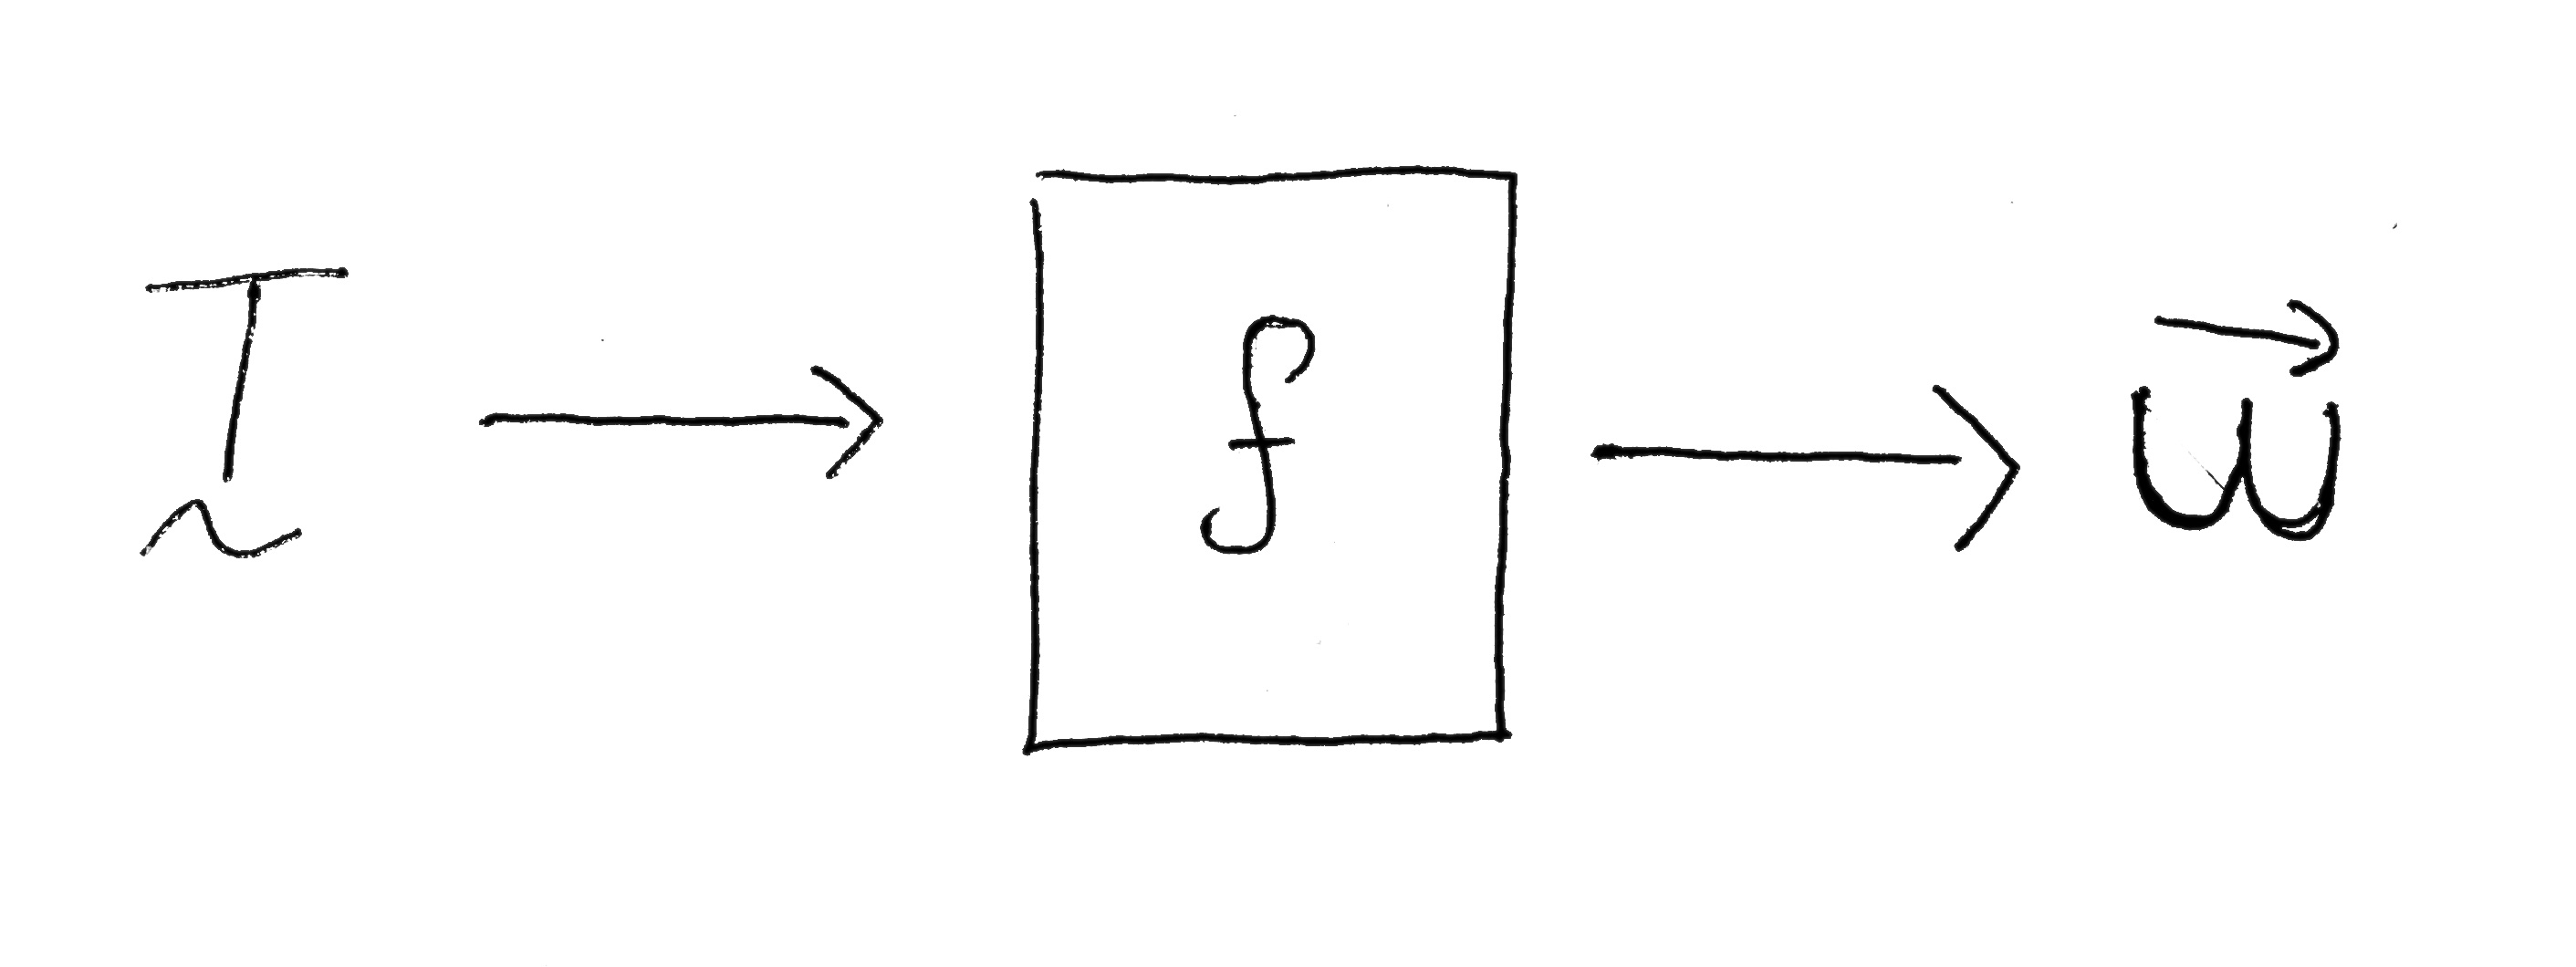
\includegraphics[width=0.45\textwidth]{recursos/machine.jpg}\par
	\vspace{1cm}
	{\scshape\Large FYS-3012 \par}
	\vspace{1.5cm}
	{\Huge\bfseries Home Exam\par}
	\vspace{2cm}
	{\Large\itshape Autumn 2017 by Arthur S. Nørve\par}

	\vfill

% Bottom of the page
	{\large 3. april 2017}
\end{titlepage}



\tableofcontents
\newpage

%#####################  CONTENT #####################



\section{Problem 1: Seal classification}

For this problem we were handed a set of 1420 vectors that represent an image of a certain type of seal (two types) after having been processed by a preliminary convolutional network. Our task is then to build a classifier that is able to separate the two types of seal, ie. separate these prerocessed vectors. Each sample consists of  4096 features so quite a lot.

\subsection{Types of classifiers and methodology}
For this problem we will take a look at five different classifiers: Bayes normal classifier assuming equal covariance (Bayes), Support Vector Machine (SVM), Least Mean Square with stochastic descent aka. Widrow-Hoff (LMS), simple least sum of squares (LS) and lastly a 2 layer perceptron algorithm (2LP). To investigate the data and reduce dimension, we'll also use principal component analysis (PCA).


\subsection{PCA analysis }
Using the PCA technique we can reduce the dimension of the data while hopefully preserving not only independent features but also group structure. As we shall see now, this is partially true.

To use the PCA, we treat our data according to the algorithm, that is: subtract the mean for the features from the training points, generate covariance matrices and collect them in the unbiased pooled covariance matrix; for two classes

\[
    \hat{\Sigma} = \frac{(n_x-1\hat{\Sigma_x}) + (n_y-1\hat{\Sigma_y})}{n_x+n_y-2}
\]

Next, we do an eigendecomposition (diagonalise) this matrix. This gives us a basis for a transformation into another space in which the features of the original data is untangled; the covariance matrix is diagonal in this space. This then gives us the possibility of cutting away dimensions with small eigenvalues; small variance. Arranging the basis vectors by the size of their eigenvalue we then select the ones we need. To investigate we look a the cumulative percentages of the sorted eigenvalues; how much the top n values contribute to the overall sum. The graph of this cumulative sum is shown in the figure below.

\begin{figure}[H]
    \centering
    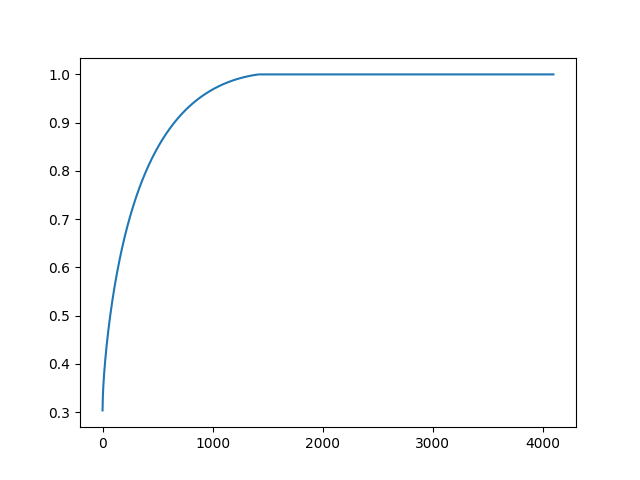
\includegraphics[width=0.6\textwidth]{recursos/1/cumsum_eigen_pca}
    \caption{Cumulative sum of sorted eigenvalues, $cutoff=1218$}
\end{figure}

What is clear here is that there is a certain part of the top vectors that contribute massively to the overall variance. The top 1218 values actually give us 0.99\% of the total. This indicates that we can shave of some dimensions to lighten our data. A further problem that we'll come across is the fact that some of our classifiers are particularily bad with high dimensions, so it might be wise and necessary to reduce the dimension further. Next up we'll take a look at what the data looks like when we reduce the dimension to two. This (obviously) allows us to take a look at the data directly in a 2D plot.

\begin{figure}[H]
    \centering
    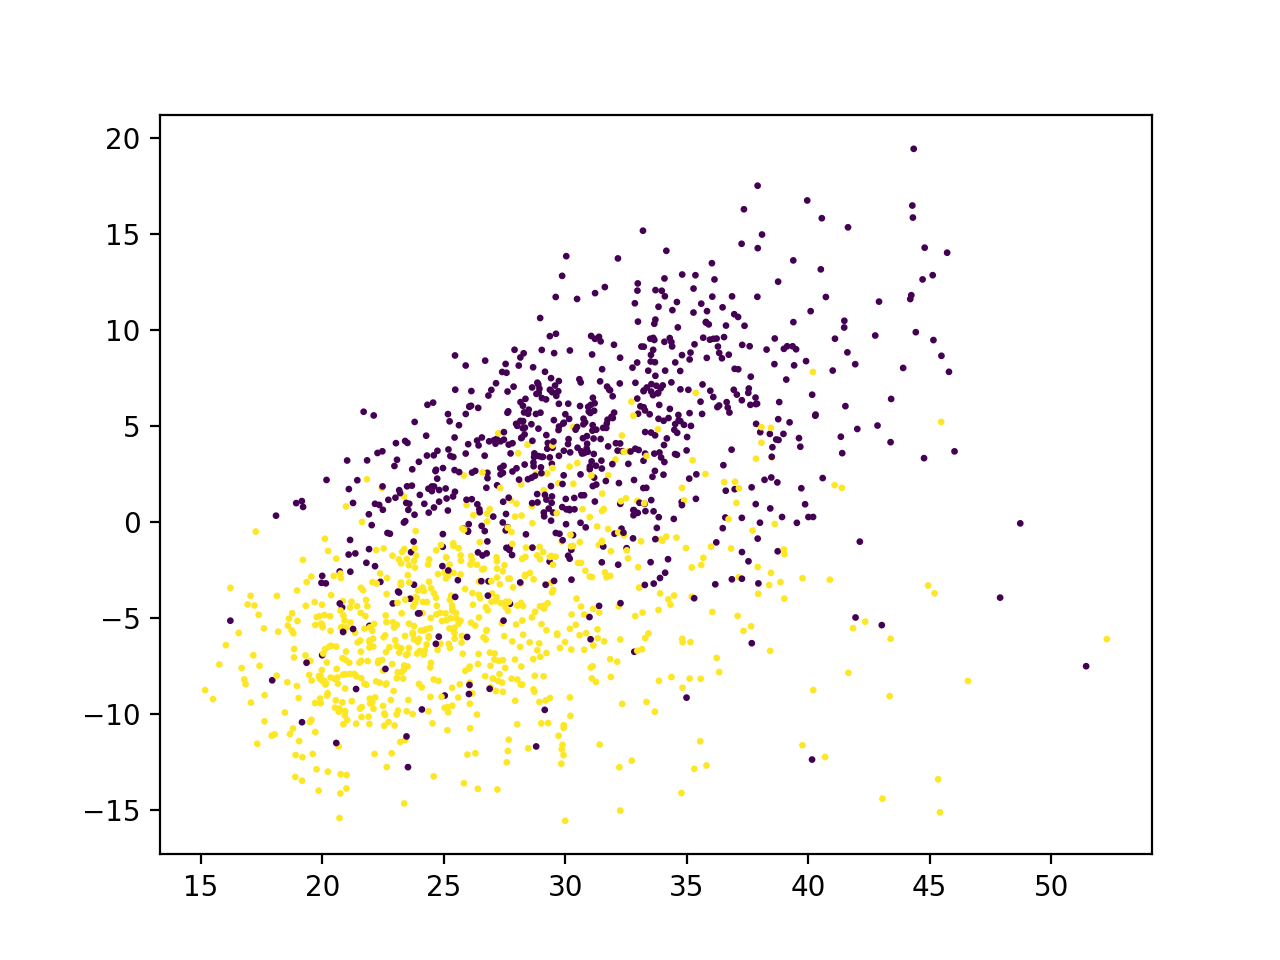
\includegraphics[width=0.7\textwidth]{recursos/1/pca_2}
    \caption{PCA dimension reduction to 2D}
\end{figure}


\subsection{Comparing classifiers across dimension and resampling }
To see how the different classifiers behaved when we changed the ratio of training data to  validation and test sets, we ran all the algorithms except for the 2LP through 10 runs each for the following ratios: 40\%, 60\% and 80\%. We kept the ratio of validation to test data at 50\%. For each run, the classifiers that needed a priori parameter settings (hyper parameters) were first taken through an optimisation stage. In this stage we first trained with a range of different values (learning rate), then validated on the validation set to check accuracy, at last we selected the parameter that yielded the highest accuracy and used that for the training. All this was done for three choices of dimension: two, the PCA threshold (99\%)  dimension; 1214 and lastly the full set (4096).

Some things can be noted before we take a look at the results. Already before we ran the classifiers we suspected that the Bayes and LS classifiers would struggle with higher dimensions. For the LS classifier the problem is that there is not an unique solution when the number of features go above the number of training points. This was confirmed as we shall soon see. The next figure shows normal distributions generated from the mean and variance of the accuracy for the ten runs.

Although not seen immediately we can extract some info from these graphs. 40\% simply isn't enough training data; this split doesn't deliver a training set large enough to give the classification algorights a satisfactory "feeling" for the data. 60\% is in most of the cases better than 40\% but still falls short of the 80\% which mostly leads (in the mean). Another observation is that the LS classifier lies around 50\% for all dimension except 2, indication what we mentioned above. The same goes for the Bayes classifier. Later we'll take a look at a graph that ilustrates the degradation that happens for these algorithms in high dimensions.


\begin{figure}[H]
    \centering
    \begin{subfigure}{0.3\textwidth}
        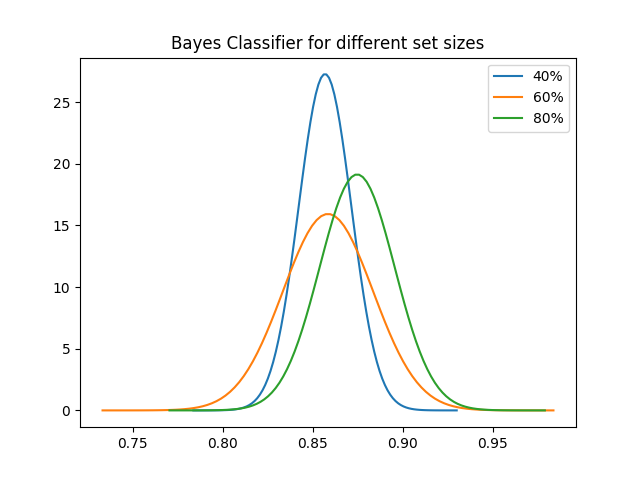
\includegraphics[width=\textwidth]{recursos/1/bayes_2}
        \caption{Bayes with two dim}
    \end{subfigure}
    \begin{subfigure}{0.3\textwidth}
        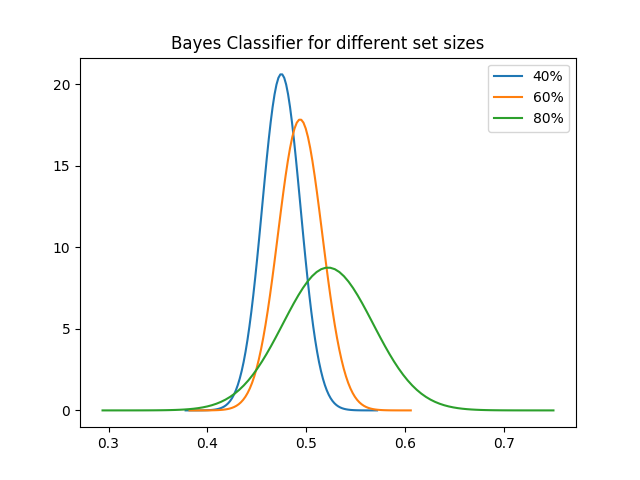
\includegraphics[width=\textwidth]{recursos/1/bayes_pca}
        \caption{Bayes with PCA dim}
    \end{subfigure}
    \begin{subfigure}{0.3\textwidth}
        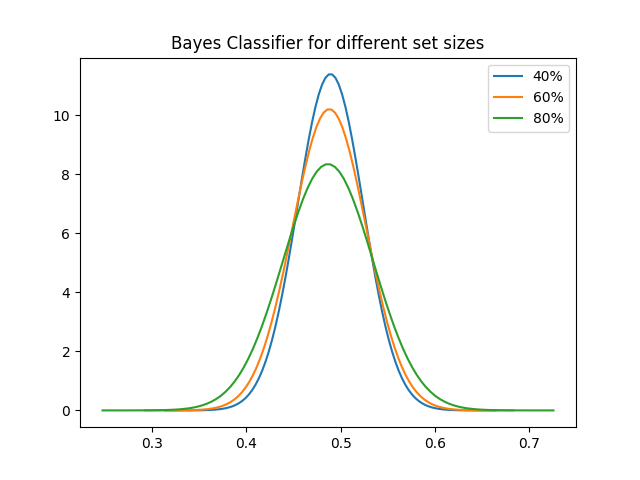
\includegraphics[width=\textwidth]{recursos/1/bayes_full}
        \caption{Bayes with full dim}
    \end{subfigure}
    ~
    \begin{subfigure}{0.3\textwidth}
        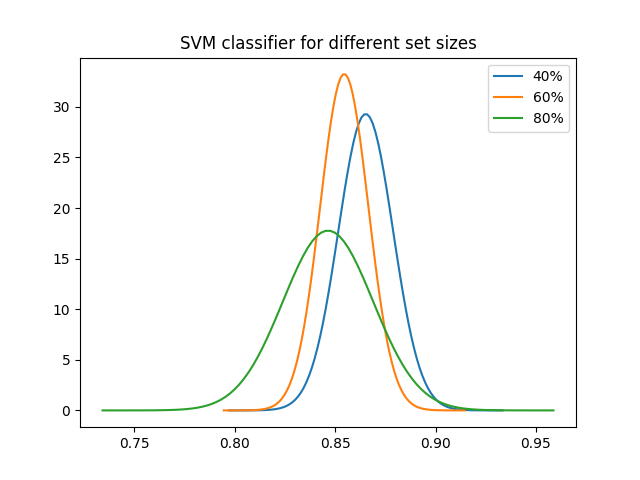
\includegraphics[width=\textwidth]{recursos/1/svm_2}
        \caption{SVM with two dim}
    \end{subfigure}
    \begin{subfigure}{0.3\textwidth}
        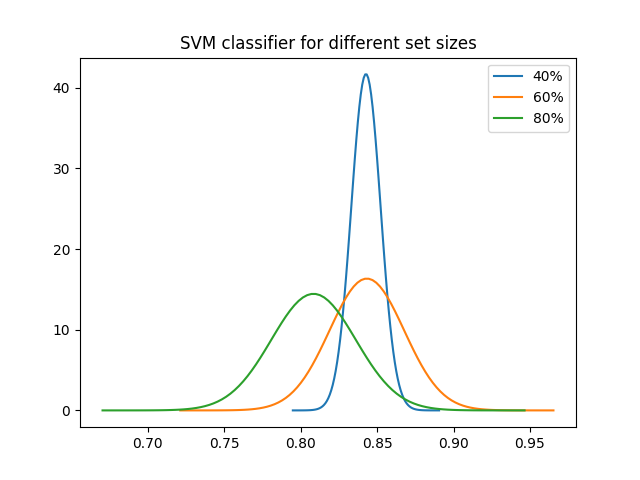
\includegraphics[width=\textwidth]{recursos/1/svm_pca}
         \caption{SVM with PCA dim}
    \end{subfigure}
    \begin{subfigure}{0.3\textwidth}
        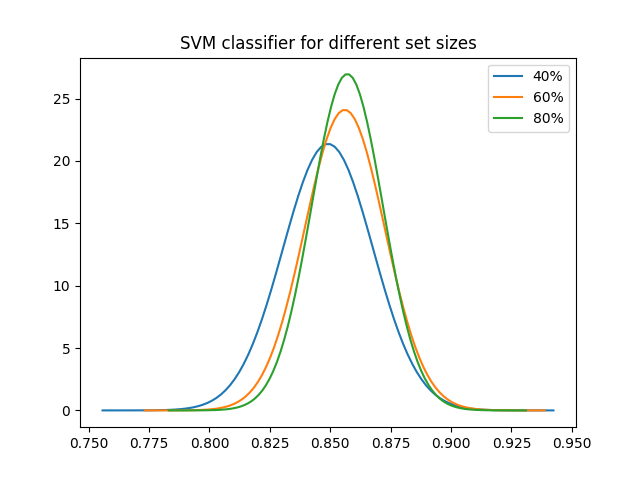
\includegraphics[width=\textwidth]{recursos/1/svm_full}
        \caption{SVM with full dim}
    \end{subfigure}
    ~
    \begin{subfigure}{0.3\textwidth}
        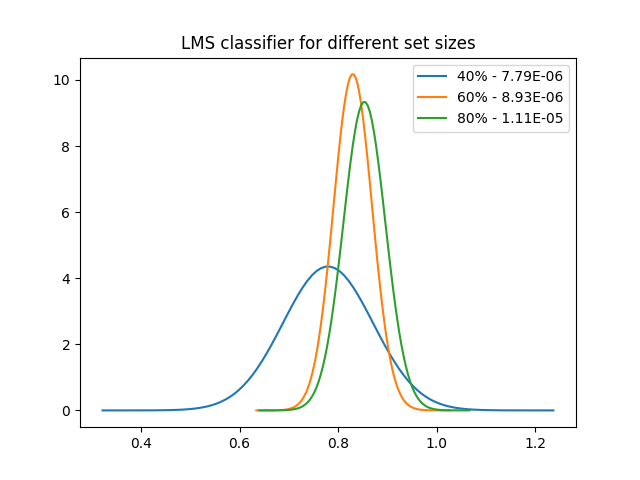
\includegraphics[width=\textwidth]{recursos/1/lms_2}
        \caption{LMS with two dim}
    \end{subfigure}
    \begin{subfigure}{0.3\textwidth}
        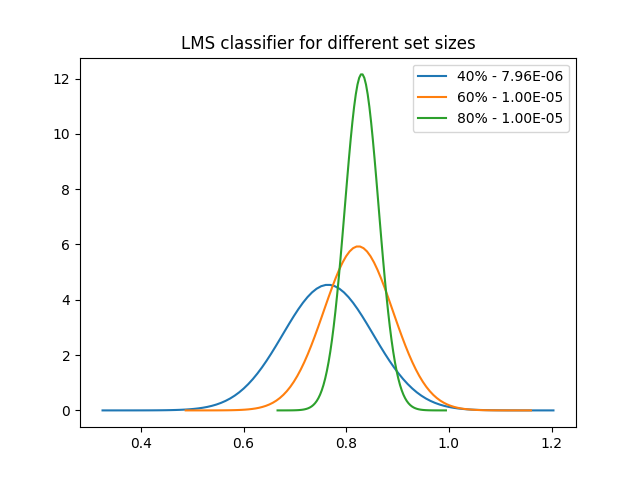
\includegraphics[width=\textwidth]{recursos/1/lms_pca}
         \caption{LMS with PCA dim}
    \end{subfigure}
    \begin{subfigure}{0.3\textwidth}
        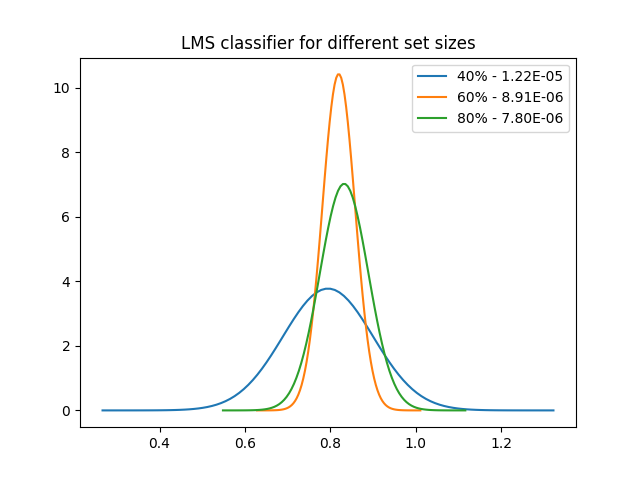
\includegraphics[width=\textwidth]{recursos/1/lms_full}
        \caption{LMS with full dim}
    \end{subfigure}
    ~
    \begin{subfigure}{0.3\textwidth}
        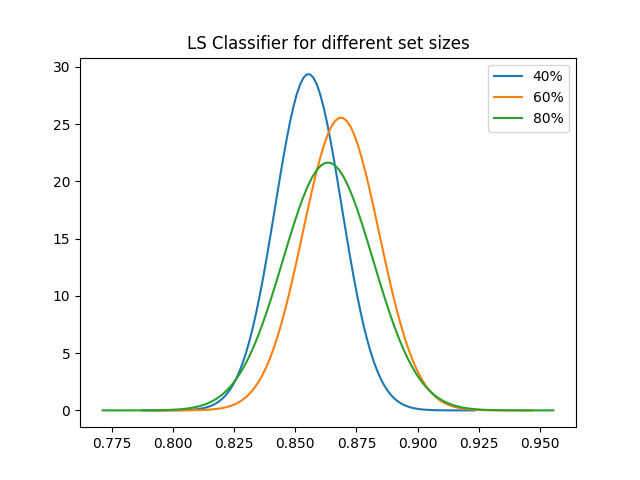
\includegraphics[width=\textwidth]{recursos/1/ls_2}
        \caption{LS with two dim}
    \end{subfigure}
    \begin{subfigure}{0.3\textwidth}
        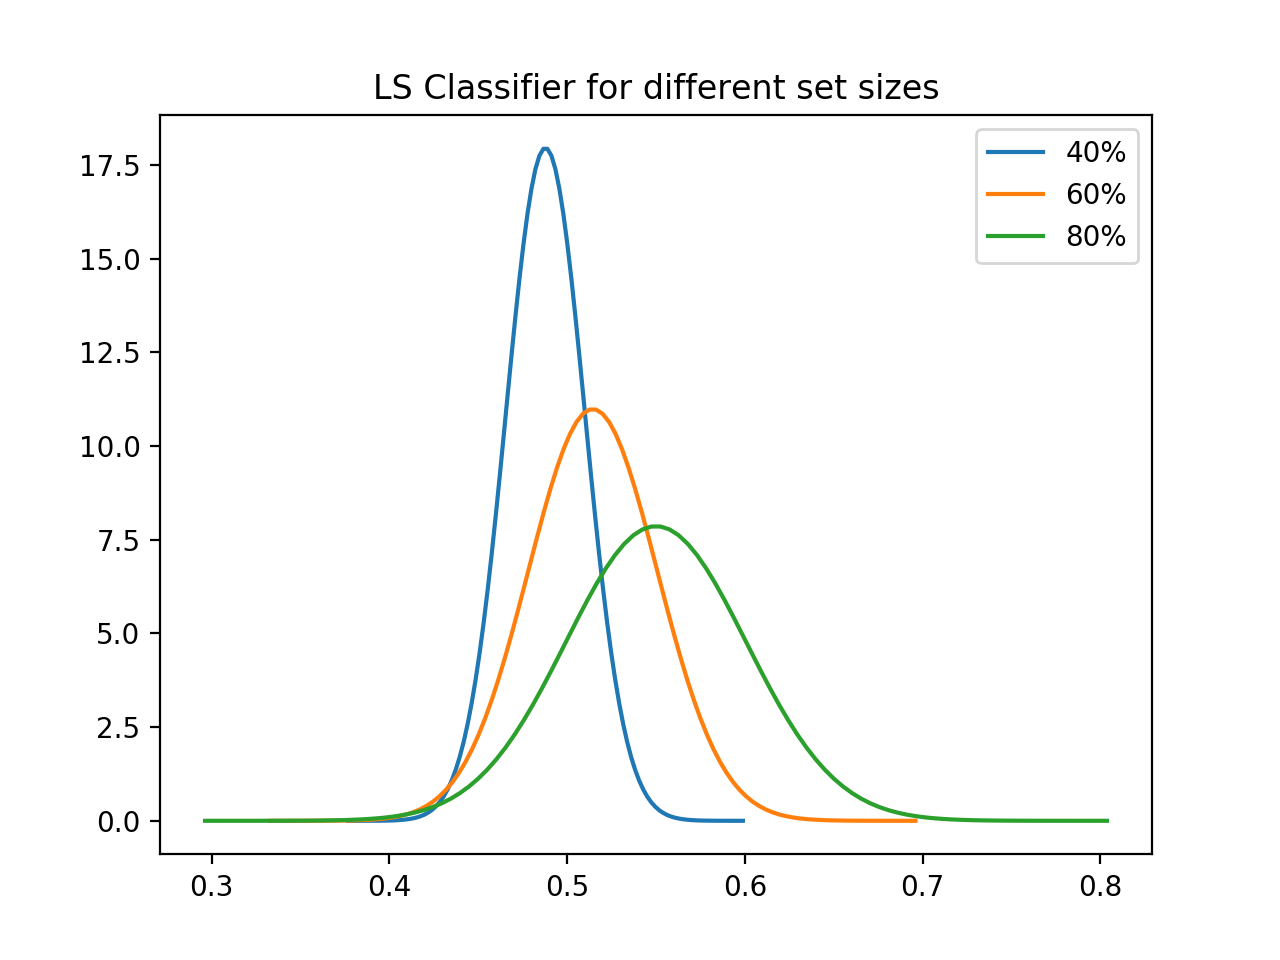
\includegraphics[width=\textwidth]{recursos/1/ls_pca}
         \caption{LS with PCA dim}
    \end{subfigure}
    \begin{subfigure}{0.3\textwidth}
        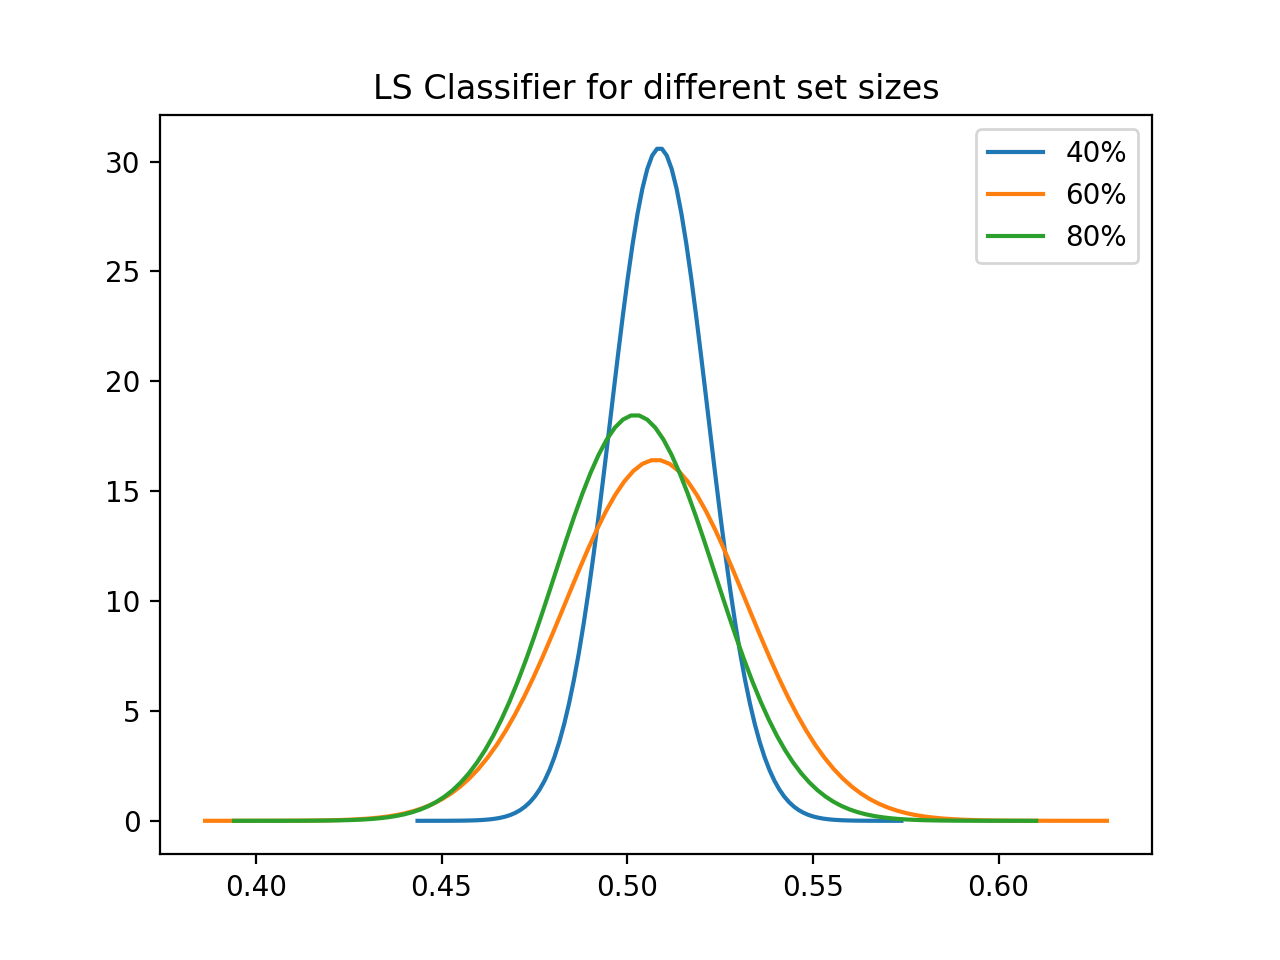
\includegraphics[width=\textwidth]{recursos/1/ls_full}
        \caption{LS with full dim}
    \end{subfigure}
    \caption{ Plots of normal distributions extrapolated from 10 runs of the classifiers with three different set ratios: 40\%, 60\% and 80\%. The number in the legend for LMS is the choosen best learning rate. }
\end{figure}

Based on the above we will use a split ratio of 70\% for the final test and further investigation. Now we'll take a brief look at what happens to the different algorithms when we increase the number of features. 
\begin{figure}[H]
    \centering
    \begin{subfigure}{0.45\textwidth}
        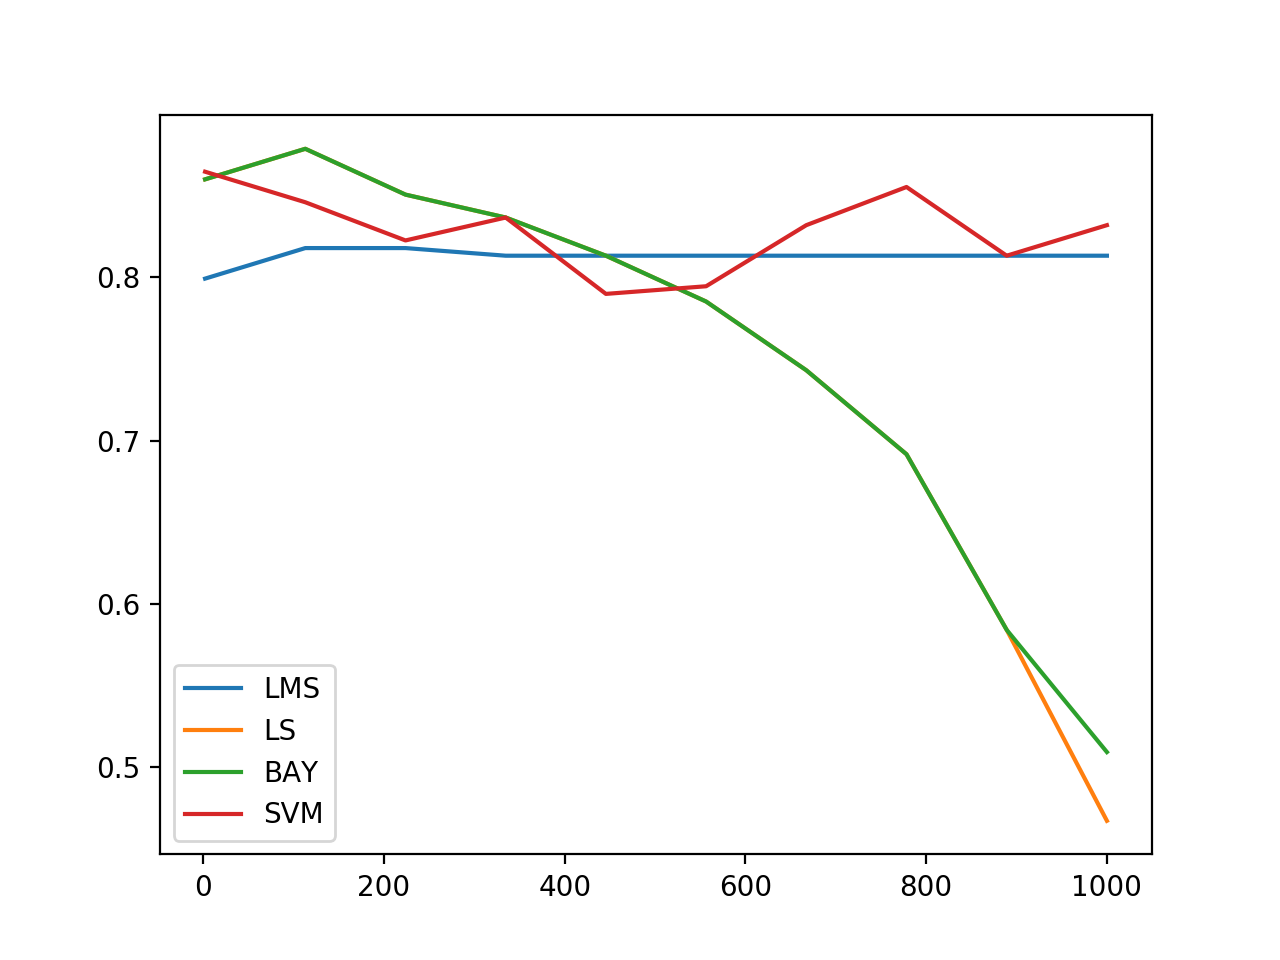
\includegraphics[width=\textwidth]{recursos/1/class_vs}
        \caption{ Without SMV. 10 dims between 2 and 1000}
    \end{subfigure}
    \begin{subfigure}{0.45\textwidth}
        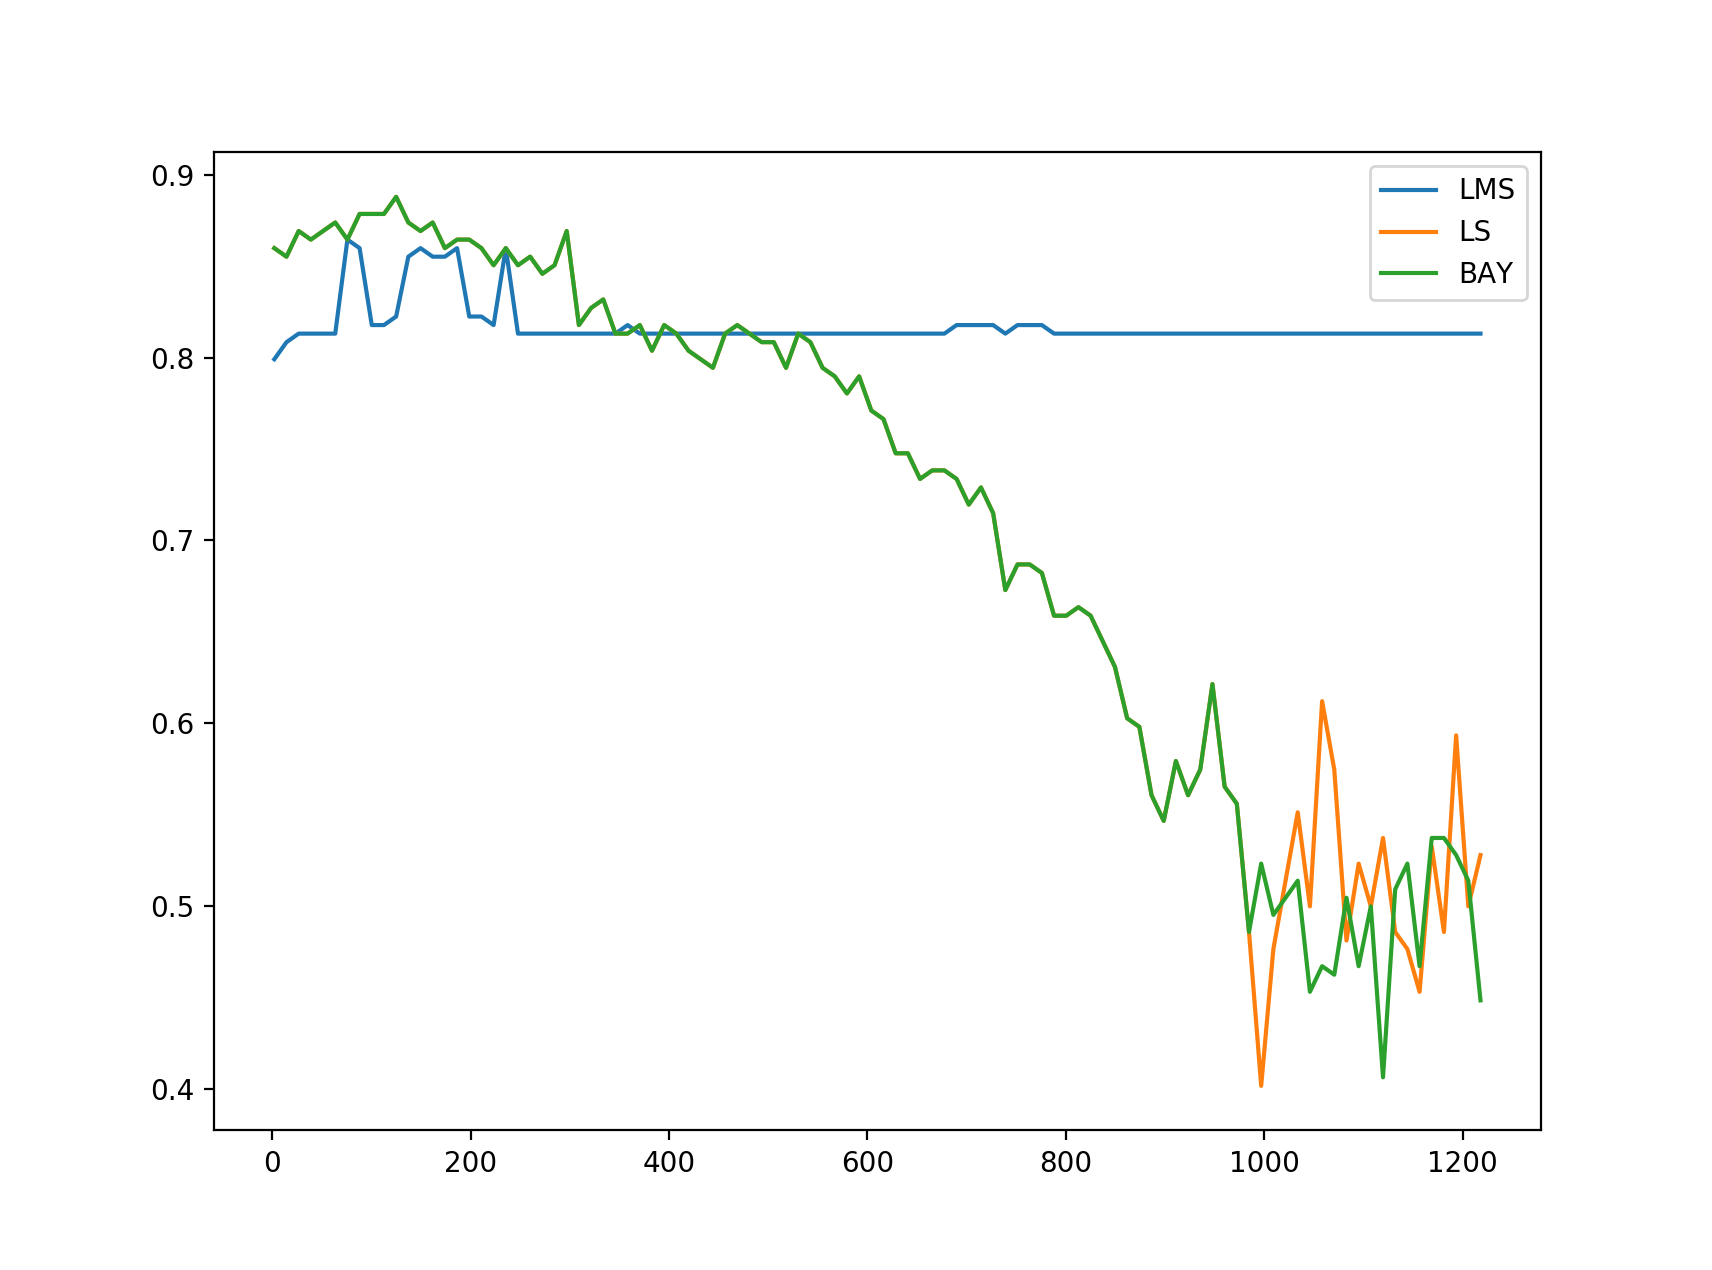
\includegraphics[width=\textwidth]{recursos/1/class_vs_simple}
        \caption{With SMV. 100 dims between 2 and 1218 }
    \end{subfigure}
     \caption{Accurcacy over dimension}
\end{figure}

Taking a look at this figure it is clear that the performance of LS and Bayes plumets as soon as the dimensions start to get "high". It is notable however that the LMS manages to stay good for as long as it does.



\subsection{Neural network: 2LP}
For the two layuer perceptron we implemented a general version but only tested four configurations due to computational time: 10 neuron network for 2d data (after PCA), 10 neuron network for original data, 50 neuron network for original data and 100 neuron network for original data. Because of the way the code is made, the networks automatically saves its state (weights and cost history) when it finishes the current iterations. Using this we set the iterations to around 2000 at a time and then manually adjustet the learning rate and momentum as the cost went down. Some runs caused the network to go dead; the cost flatlines as all weights are pushed to zero and unable to recover because of the Relus zero gradient there. This is one of the common artefacts of the Relu, some solutions are modifying the Relu function, and use exponential/noisy/leaky relu, but these don't match the relu in speed since there is virtually no computations (arithmetic operations) involved. When we saw that the neurons died we terminated the run and lowered the learning rate. After a couple of runs the cost starts to slow its decline and occilate at the same time, to counter this we played with the momentum as well. Eventually we ended up with networks that on average have an accuracy in the mid 80\% range, ie. the same as for the other methods. We will now take a look at the cost functions for three of our networks: the 10 neuron for 2d data and the 50 and 100 neuron networks for full data.

\begin{figure}[H]
    \centering
    \begin{subfigure}{0.3\textwidth}
        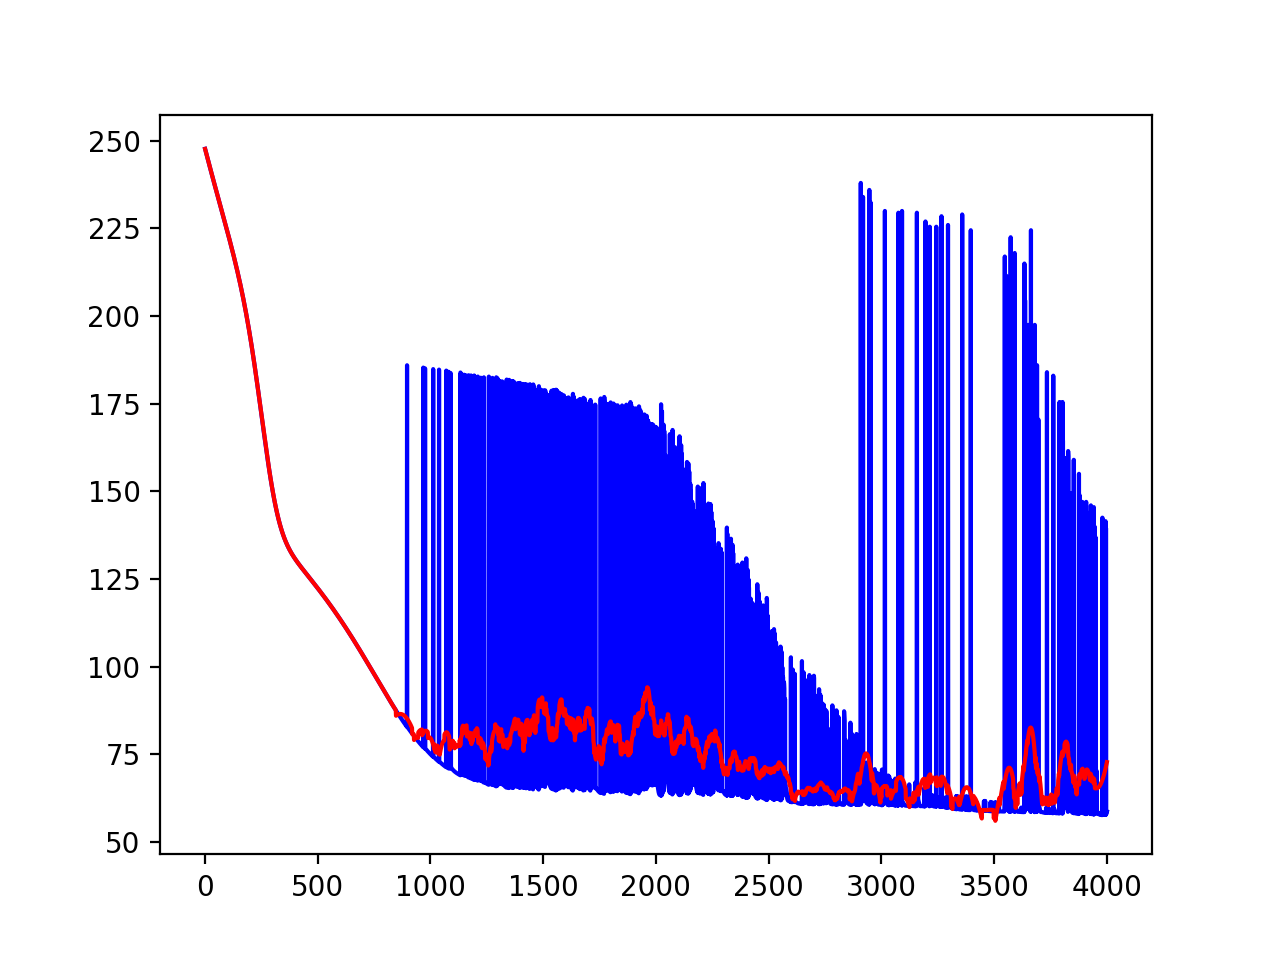
\includegraphics[width=\textwidth]{recursos/1/cost_10_2d}
        \caption{10 neurons trained on 2d data}
    \end{subfigure}
    \begin{subfigure}{0.3\textwidth}
        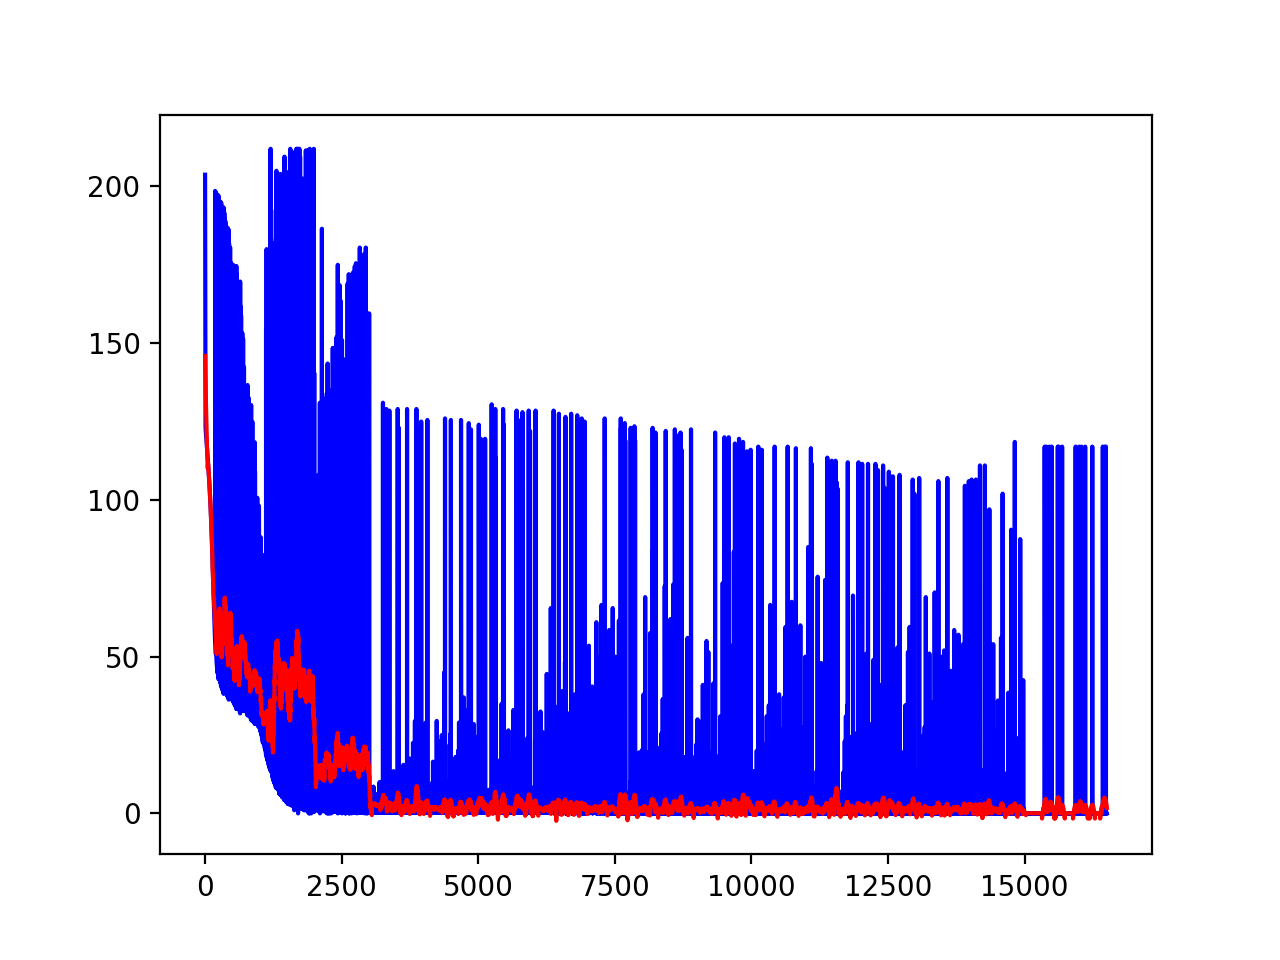
\includegraphics[width=\textwidth]{recursos/1/cost_50}
        \caption{50 neurons trained on full dim data}
    \end{subfigure}
    \begin{subfigure}{0.3\textwidth}
        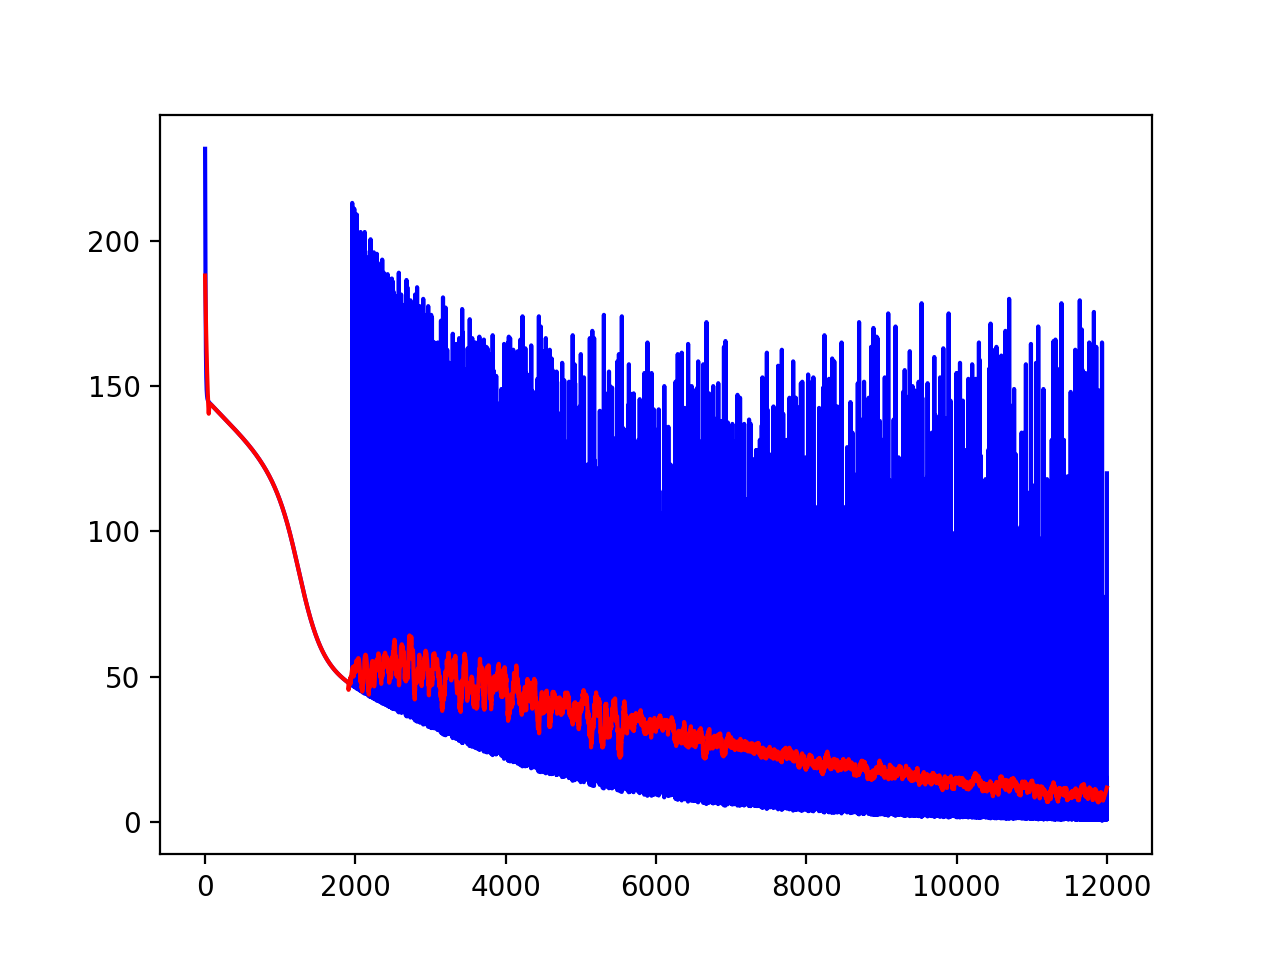
\includegraphics[width=\textwidth]{recursos/1/cost_100}
        \caption{100 neurons trained on full dim data}
    \end{subfigure}
     \caption{Cost over number of iterations, the red line is the cost (blue) that has been processed by a Savitzky-Golay filter (99 samples as window size) to smooth it out.}
\end{figure}

As can be seen from the plots the fluctuations are major, but then again, the networks weren't taken through that many iterations. More could have been done here, I would for example have liked to be able to adjust layer size (number of neurons) and learning rate using cross-validation on a separate valiation set, just like for LMS. The problem is that it would have taken me a week to go through all the values and have networks with converging cost.



\subsection{Conclusion }
In general one can see than on average, the Bayes classifier is doing really well. Across dimensions it quickly dies in favour for the much more reliable (for "high" dims) LMS. To extend, taking a look at Langranian Eigenmaps and some other transformation techniques might have been fruitful. The network; the 2LP could also have been tested more.

\section{Problem 2: Chlorophyll contents regression}
For this task we are given a data set with vectors representing pixel from a multiband satelite image. The corresponding values ('labels') are then the true meassure of chlorophyll content in the given pixels in some units. The task is then to use regression to estimate the chlorophyll contents of an unknown pixel given a new one. In the task it is specified that this is to be done with a cross-validation method called leave one out (LOO), that is we're supposed to remove one sample, then train on the remaining 134 samples and see what we get. We have done this using LMS with stochastic descent and a simple LS regression.


\subsection{LMS Regression}
\begin{figure}[H]
    \centering
    \begin{subfigure}{0.45\textwidth}
        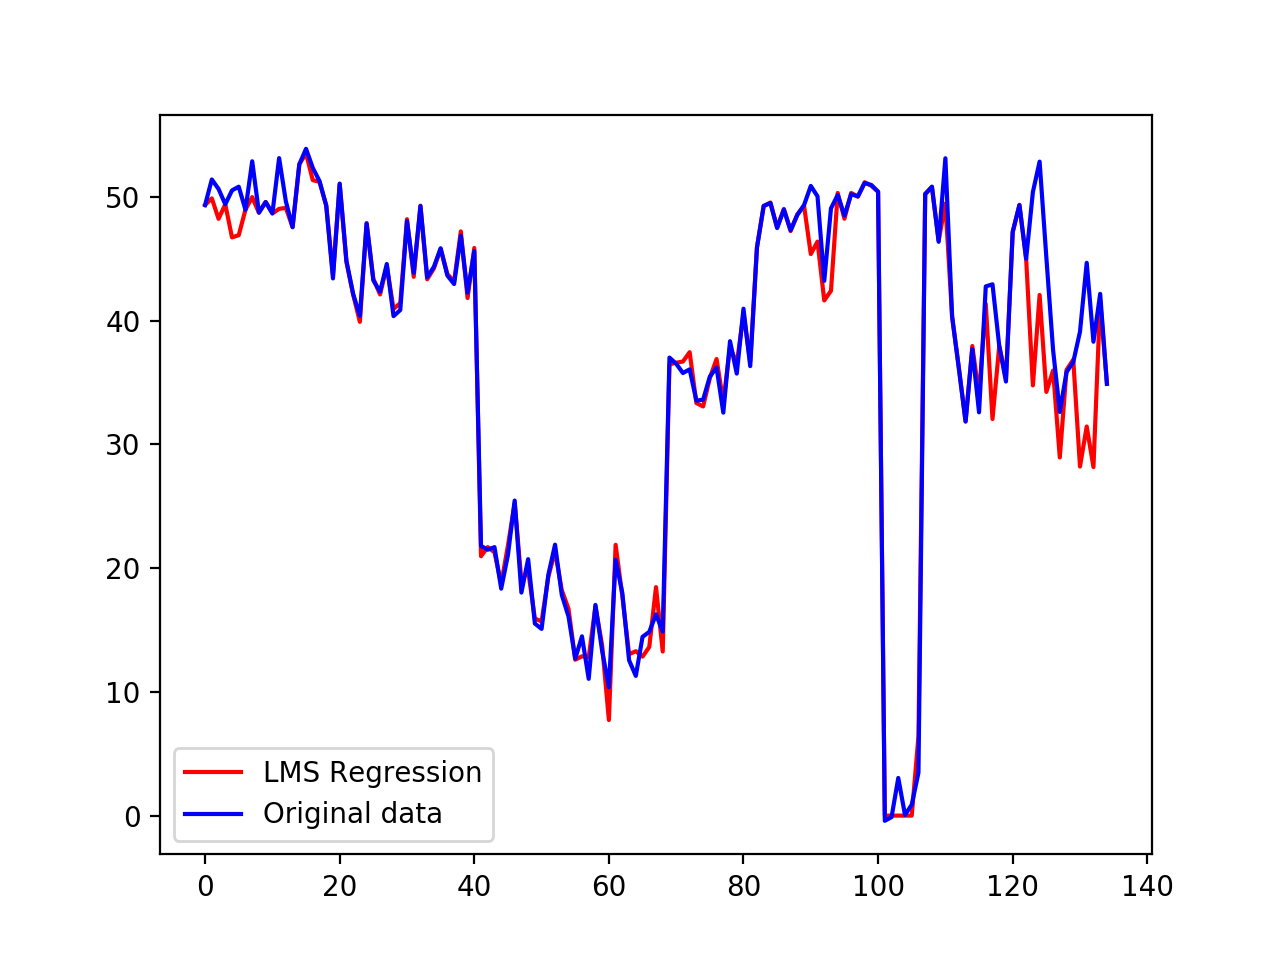
\includegraphics[width=\textwidth]{recursos/2/lms_regression_individual_tune}
        \caption{ Individual tuning}
    \end{subfigure}
    \begin{subfigure}{0.45\textwidth}
        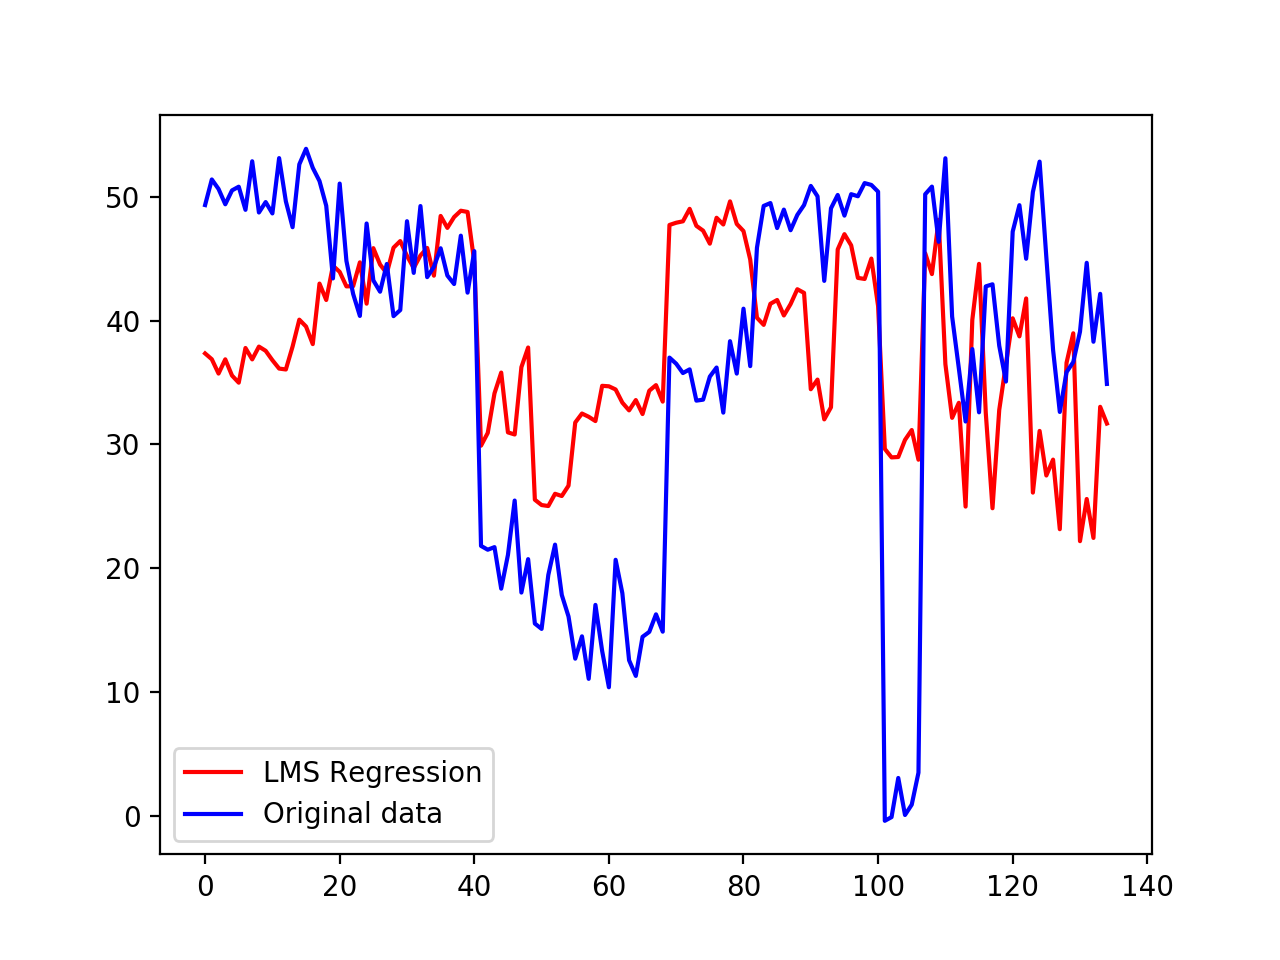
\includegraphics[width=\textwidth]{recursos/2/lms_regression_global_tune}
        \caption{ Global tuning}
    \end{subfigure}
     \caption{LMS regression for the chlorophyll data.}
\end{figure}

For the LMS regression we tried to test two different possible tuning scenarios of the learning rate in the first graph you see the result of tuning the learning rate each time for each point left out. That is the learning rate was set so that the squared error for the one left out point was minimised each time. In this case the total squared difference was $1243.84$ and the average learning rate used for all points was $\bar{\rho} = 1.216*10^{-10}$. In the second graph you see the result of the regression where the learning rate has been optimised before the regression took place. That is that the entire procedure was tested for different learning rates, and the value that minimised the overall squared error was selected and used for the regression showed in the graph. The total squared difference was $22573.1$ using the learning rate $\rho = 2.81*10^{-11}$. In the graph a) below, the individual values used for each run is shown as a function of the run number itself. In b) the total squared error as a function of the learning rate is shown. Note that the y-axis in a) is on the same order of magnitude as the x axis of b), so the minimum overall value in b) is inline with the flat section in the middle of the graph in a).


\begin{figure}[H]
    \centering
    \begin{subfigure}{0.45\textwidth}
        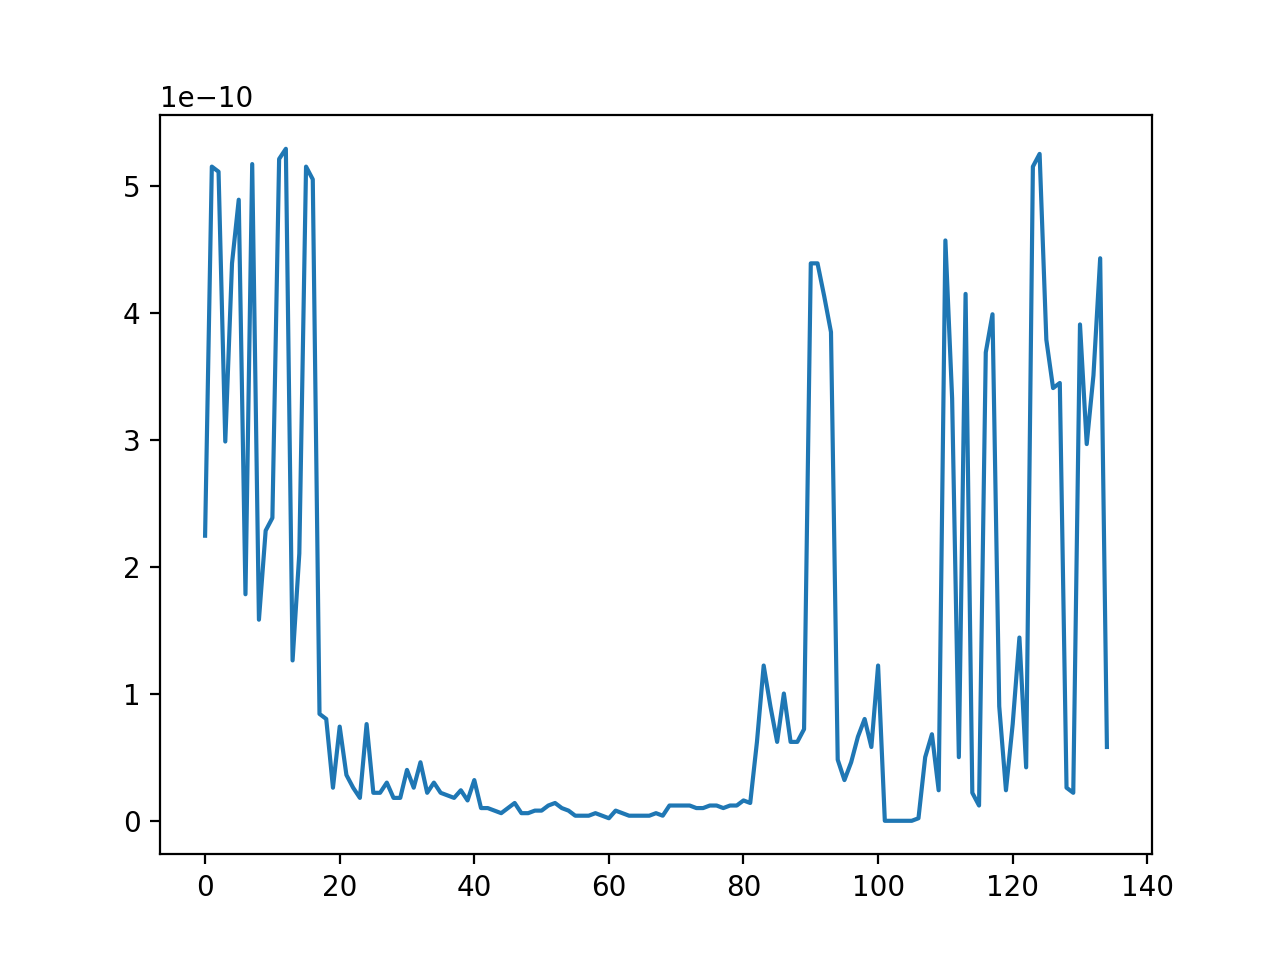
\includegraphics[width=\textwidth]{recursos/2/lms_regression_individual_mu_values}
        \caption{ Values of $\rho$ used per test  }
    \end{subfigure}
    \begin{subfigure}{0.45\textwidth}
        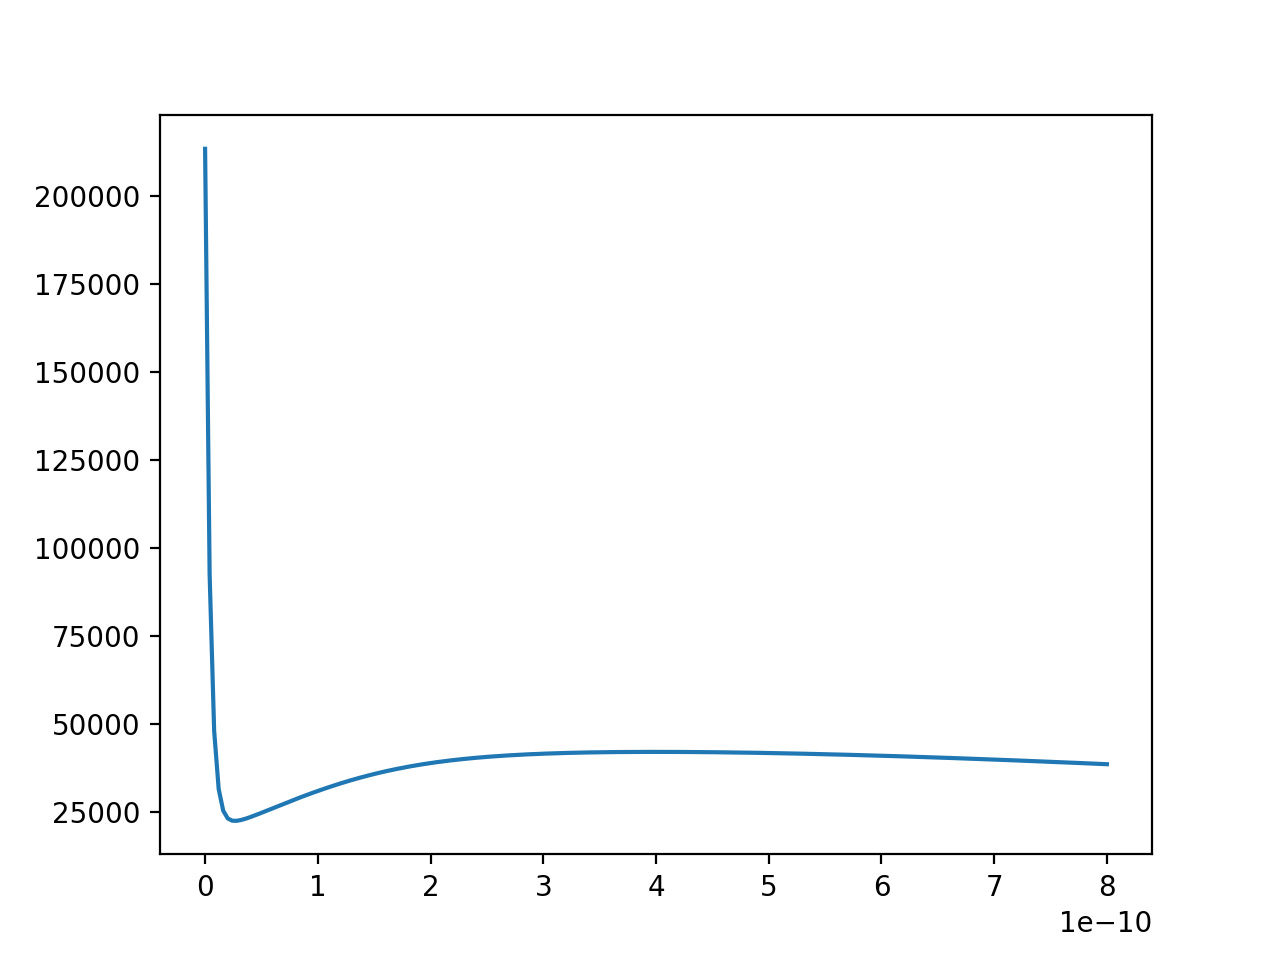
\includegraphics[width=\textwidth]{recursos/2/lms_regression_global_mu_tune}
        \caption{ Total squared error over $\rho$ }
    \end{subfigure}
     \caption{ Detailing the way the learning rate $\rho$ was set and used }
\end{figure}

\subsection{LS Regression}
Moving on we take a look at standart sum of squares regression (LS). This is implemented as is since it doesn't have any parameters to tweak and adjust. In the graph below the result of the regression can be seen. The total squared error in this case was $5496.5$, more than for the (unrealistic) individually tuned LMS, but way lower than for the normal LMS regrassion with its more than 20k total squared error.

\begin{figure}[H]
    \centering
    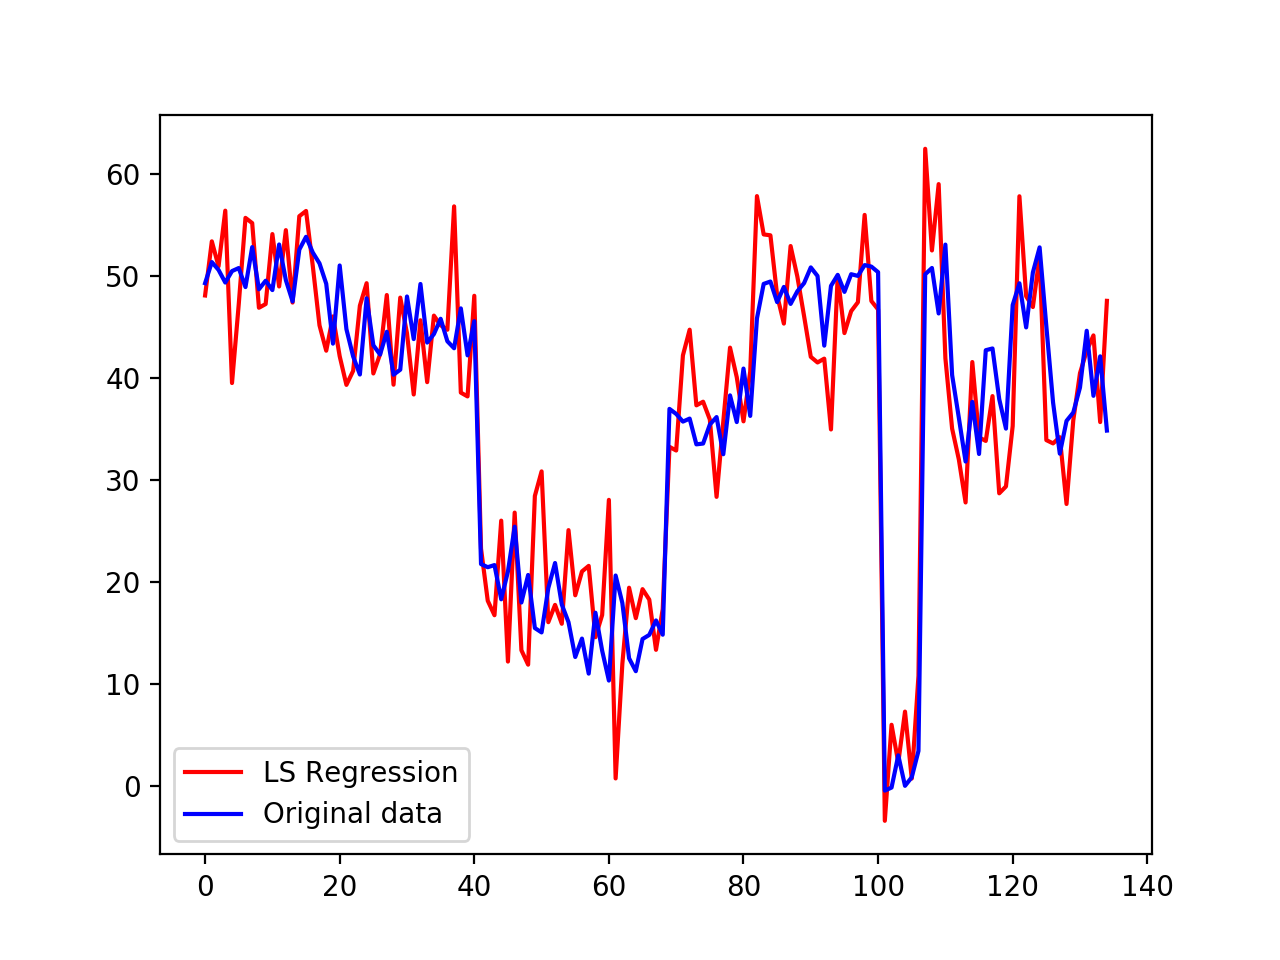
\includegraphics[width=0.6\textwidth]{recursos/2/ls_regression}
    \caption{ LS regression for the chlorophyll data }
\end{figure}

\subsection{Conclusion}
In total the LS regression seems to work best of the ones used. The individually adjusted LMS is more an experiment than anything else since it is unrealistic given the spread in learning rate. The case is that in this tuning is only so that each point in itself is classified correctly, this though says nothing about how the rest of the points are classified; it's mission is to strictly minimise for the one missing individual point.  As such, it is a lesson in a way; thinking about what one wants to minimise (optimise) for is very important...



\section{Problem 3: Binary digit classification}
in this problem we are supposed to create a classifier that is able to separate images of binary digits; two class classification. For this problem the input data is the raw pixel data from 16px by 16 px images, that makes for 256 dimensional feature vectors. We were handed two data sets: one with 10 and another with 200 points. We were also given an ordered data set consisting of points corresponding to bits of letters in an ASCII encoded message from the Gods. To begin with we will therefore investigate the data using dimensionality reduction and some simple comparisons. 

\subsection{Data investigation}
First we'll reduce to two dimensions and see what we get for both the small (10 points) and the large set (200 points). Then we'll run some classifiers on our set and see how well we do. Given the detailed exposition in problem 1, we'll be more brief here. Using PCA for both the larger and smaller data set we can reduce to the wanted dimension, for plottin we need 2 of course. First, however, we take a look at the cumulative eigenvalue contribution for the two sets:

\begin{figure}[H]
    \centering
    \begin{subfigure}{0.45\textwidth}
        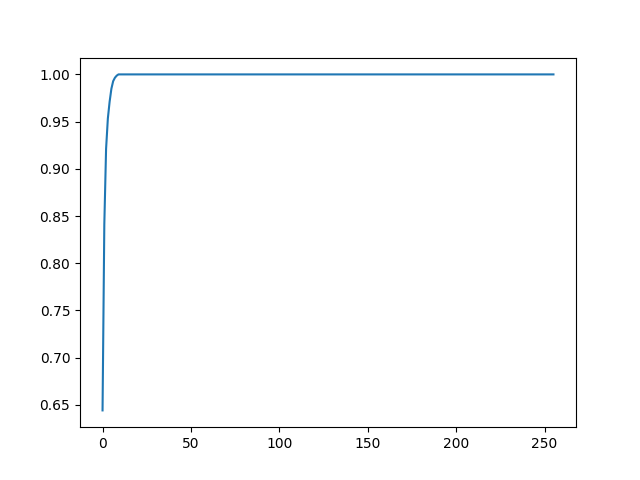
\includegraphics[width=\textwidth]{recursos/3/cumsum_eigen_pca}
        \caption{ For the small set, the $cutoff=6$ }
    \end{subfigure}
    \begin{subfigure}{0.45\textwidth}
        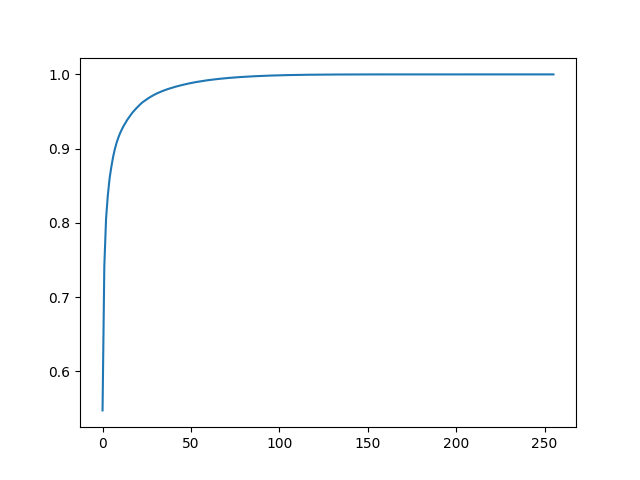
\includegraphics[width=\textwidth]{recursos/3/cumsum_eigen_pca_larger}
        \caption{ For the large set, $cutoff=54$}
    \end{subfigure}
     \caption{Cumulative sum of sorted eigenvalues}
\end{figure}

It is evident that we in both cases can reduce the dimension quite a bit, as always with PCA though, the question of whether group structure is preserved remains. Taking a look at the next two graphs, we have the answer, at least partially. It seem to be so that the two different classed form two (linearly) separable blobs of data. One is quite a bit bigger that the other though.

\begin{figure}[H]
    \centering
    \begin{subfigure}{0.45\textwidth}
        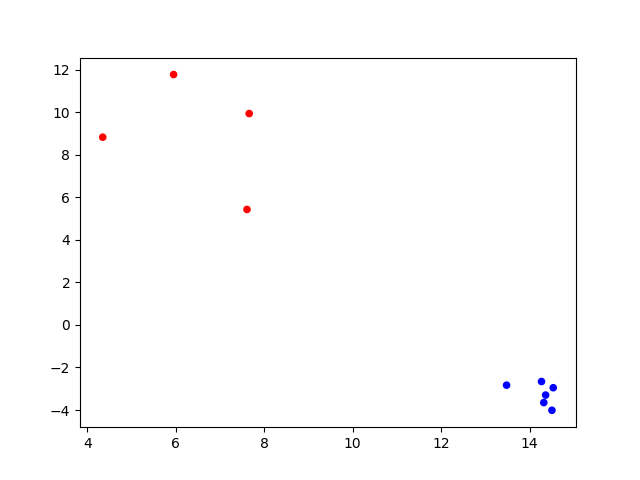
\includegraphics[width=\textwidth]{recursos/3/pca_smaller}
        \caption{ Small set in 2D using PCA }
    \end{subfigure}
    \begin{subfigure}{0.45\textwidth}
        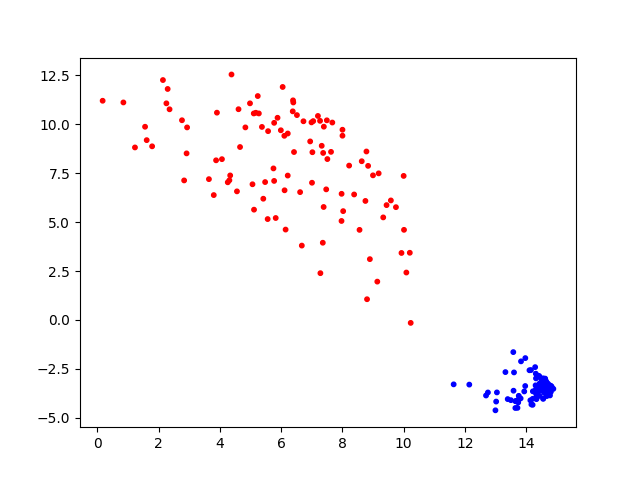
\includegraphics[width=\textwidth]{recursos/3/pca_larger}
        \caption{ Large set in 2D using PCA }
    \end{subfigure}
     \caption{The binary digit data sets in 2D after PCA dimention reduction}
\end{figure}


The next figure, enlightening as it is, was generated using the same 70\%, 15\%, 15\% split as in problem 1 because of the use of an automated procedure. That means that for the smaller set one obtains  7 training points and only 1/2 validation test points. The case is more convincing for the large set however where there is a substantial amount of vectors present for validation and testing. This is one of the reasons the small set is difficult to work with as is, and this presents itself as one of the core differences between the two: The larger naturally gives a broader perspective of the data; that is intrinsic, but 10 points (6,4 split) is in general too few. As it so happens these classifiers handle the case well, probably because of the clear linear separability of the classes.

\begin{figure}[H]
    \centering
    \begin{subfigure}{0.45\textwidth}
        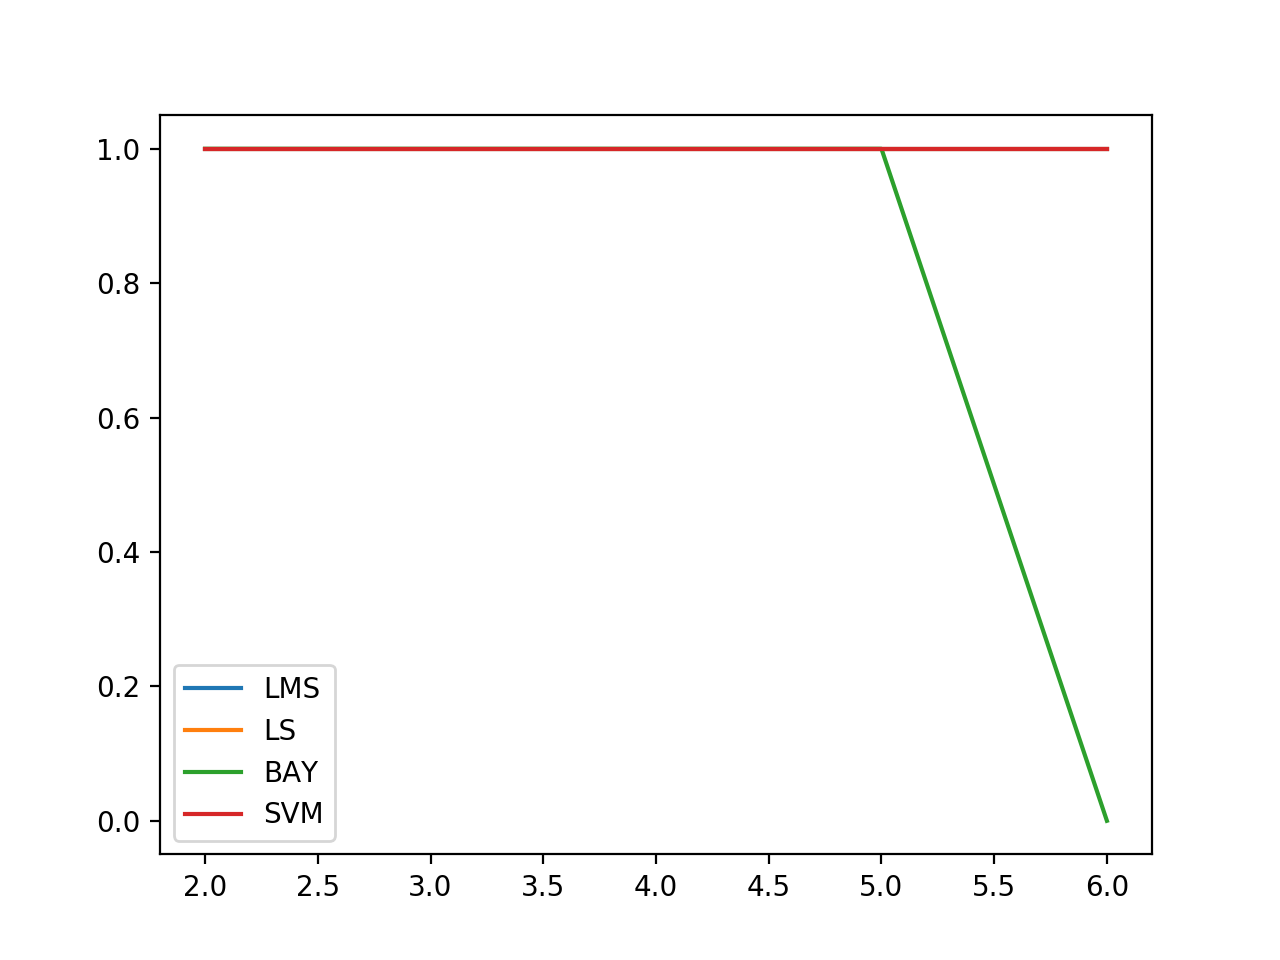
\includegraphics[width=\textwidth]{recursos/3/class_vs_small}
        \caption{ For the small set }
    \end{subfigure}
    \begin{subfigure}{0.45\textwidth}
        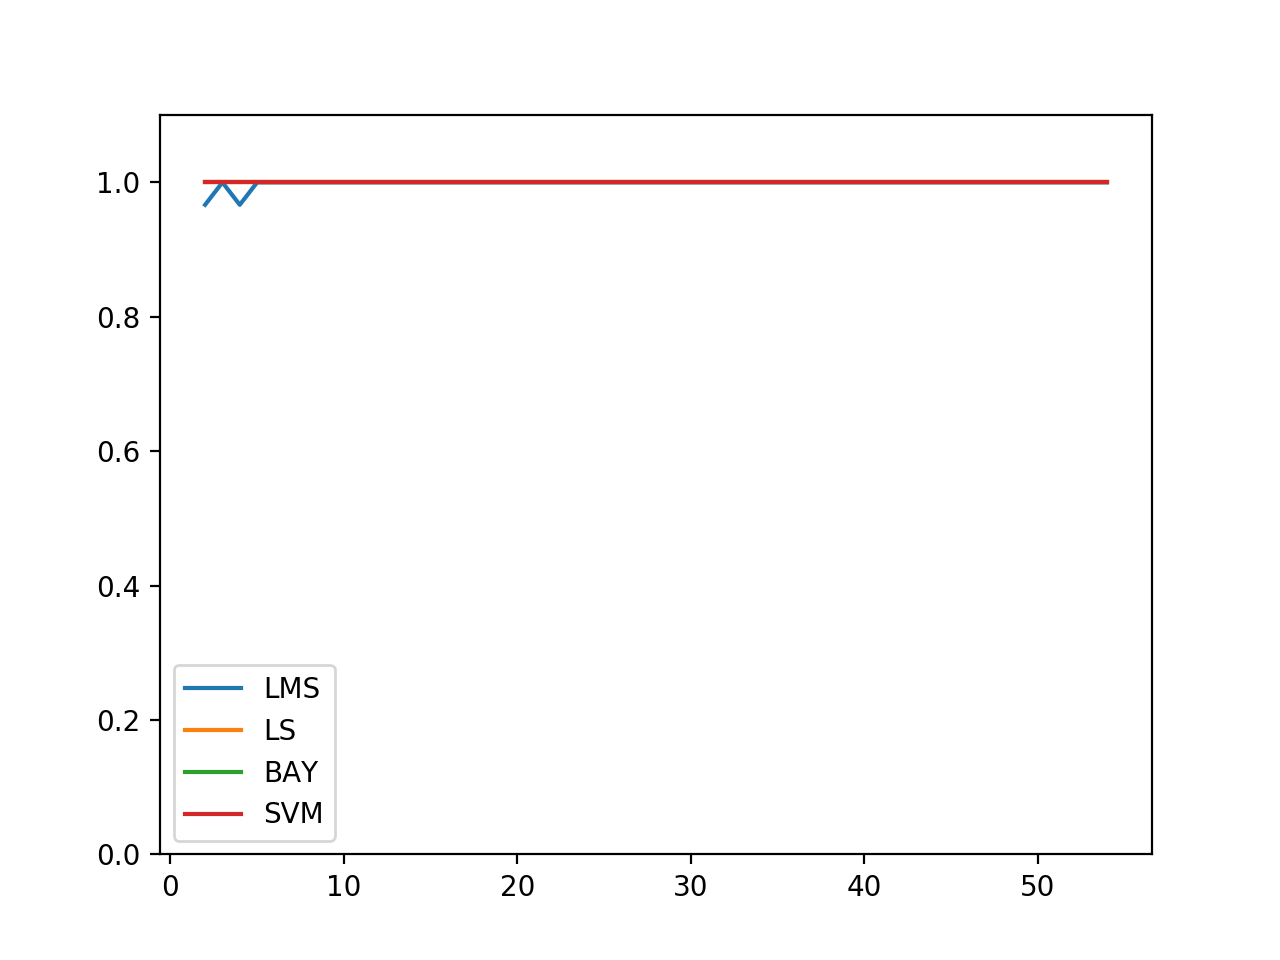
\includegraphics[width=\textwidth]{recursos/3/class_vs_large}
        \caption{ For the large set }
    \end{subfigure}
     \caption{Classifier accuracy for different dimensions}
\end{figure}

For the next insight we'll do something more relevant, namely try to train on the small set and test on the large set. Looking at the 2D plots above, one might suspect that this will yield bad results given the larger sample variance for the "red" class along one of the principal directions. Taking a look at the same kind of plot as above but for our new case we see the following:


\begin{figure}[H]
    \centering
    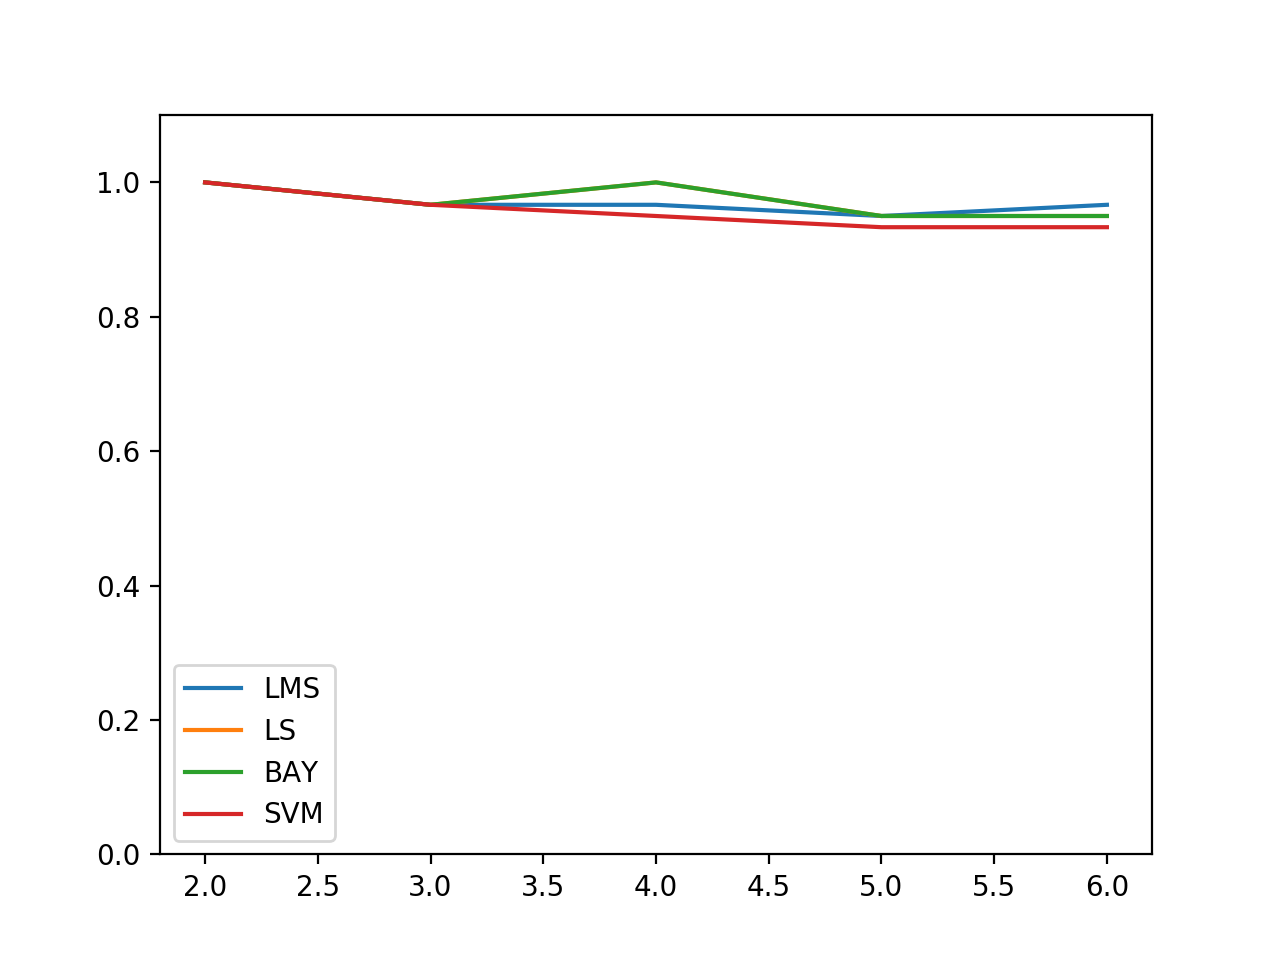
\includegraphics[width=0.7\textwidth]{recursos/3/dim_small_vs_large}
    \caption{Classifier accuracy for different dimensions with training on the small set and test on the large set.}
\end{figure}

For completeness we also show the decision boundaries for the four different methods in the graph below.

\begin{figure}[H]
    \centering
    \begin{subfigure}{0.45\textwidth}
        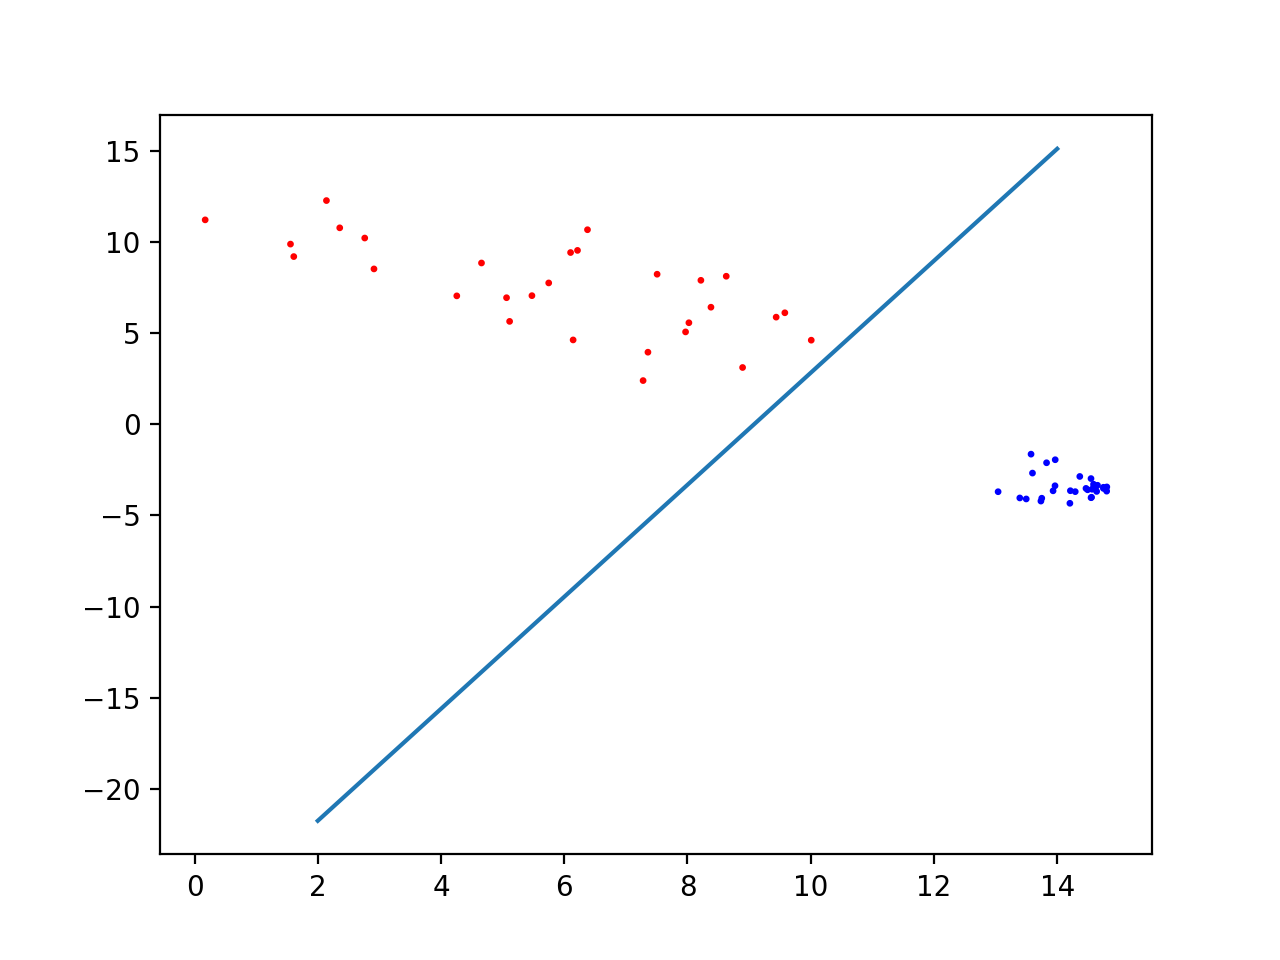
\includegraphics[width=\textwidth]{recursos/3/ls_small}
        \caption{LS}
    \end{subfigure}
    \begin{subfigure}{0.45\textwidth}
        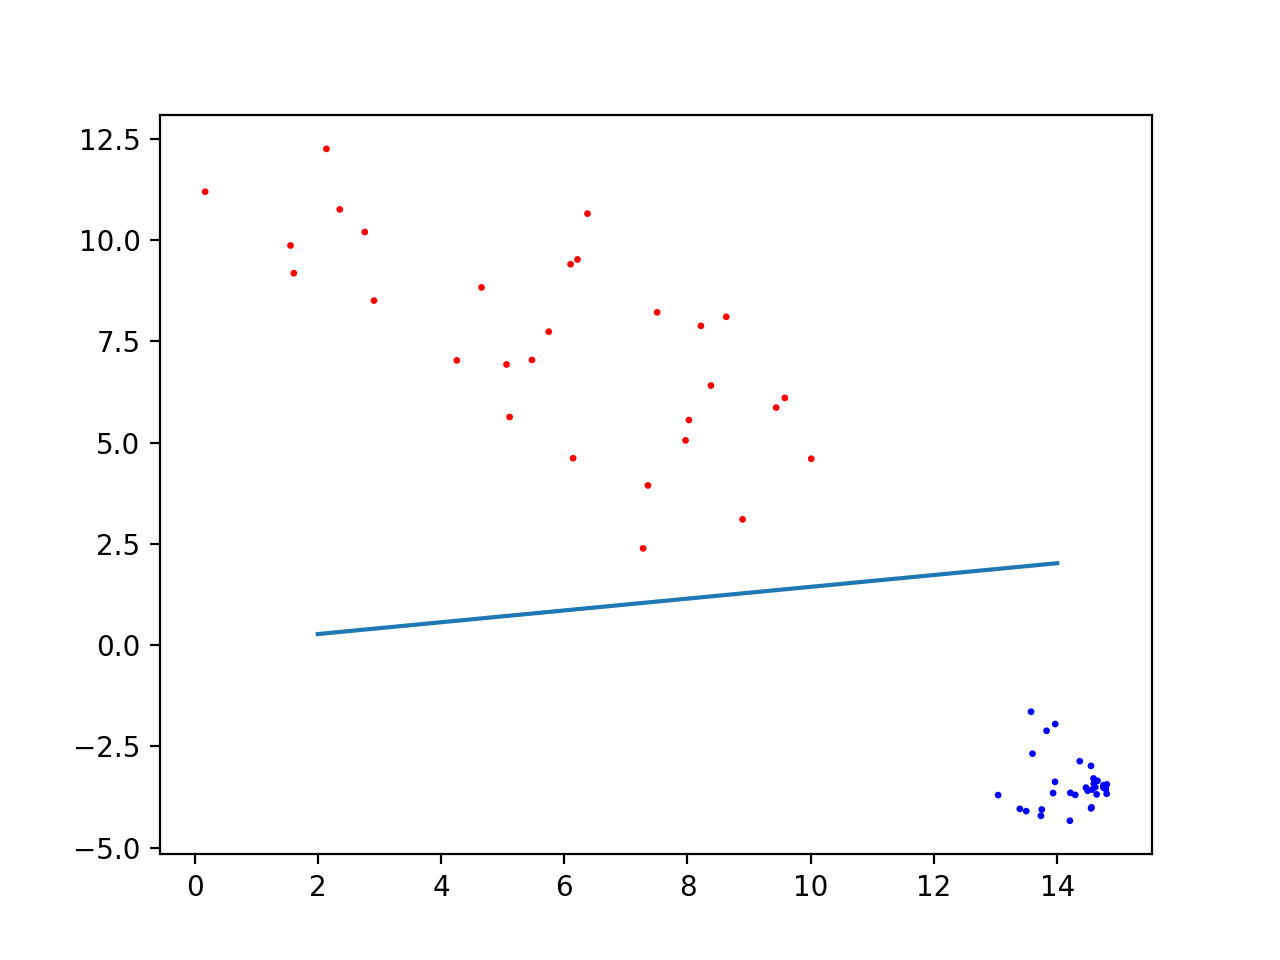
\includegraphics[width=\textwidth]{recursos/3/lms_small}
        \caption{LMS }
    \end{subfigure}
    ~
     \begin{subfigure}{0.45\textwidth}
        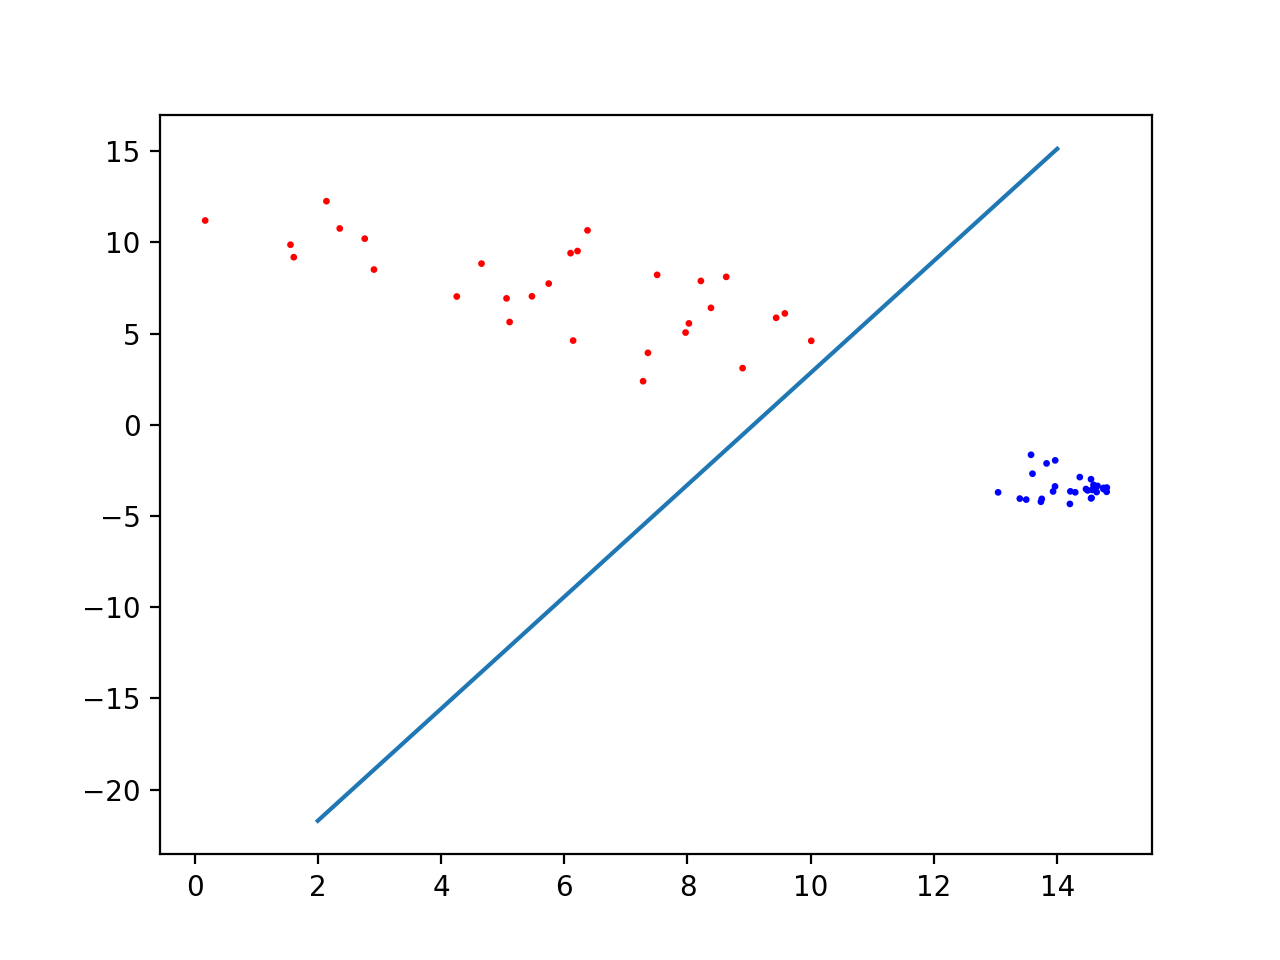
\includegraphics[width=\textwidth]{recursos/3/bayes_small}
        \caption{Bayes}
    \end{subfigure}
    \begin{subfigure}{0.45\textwidth}
        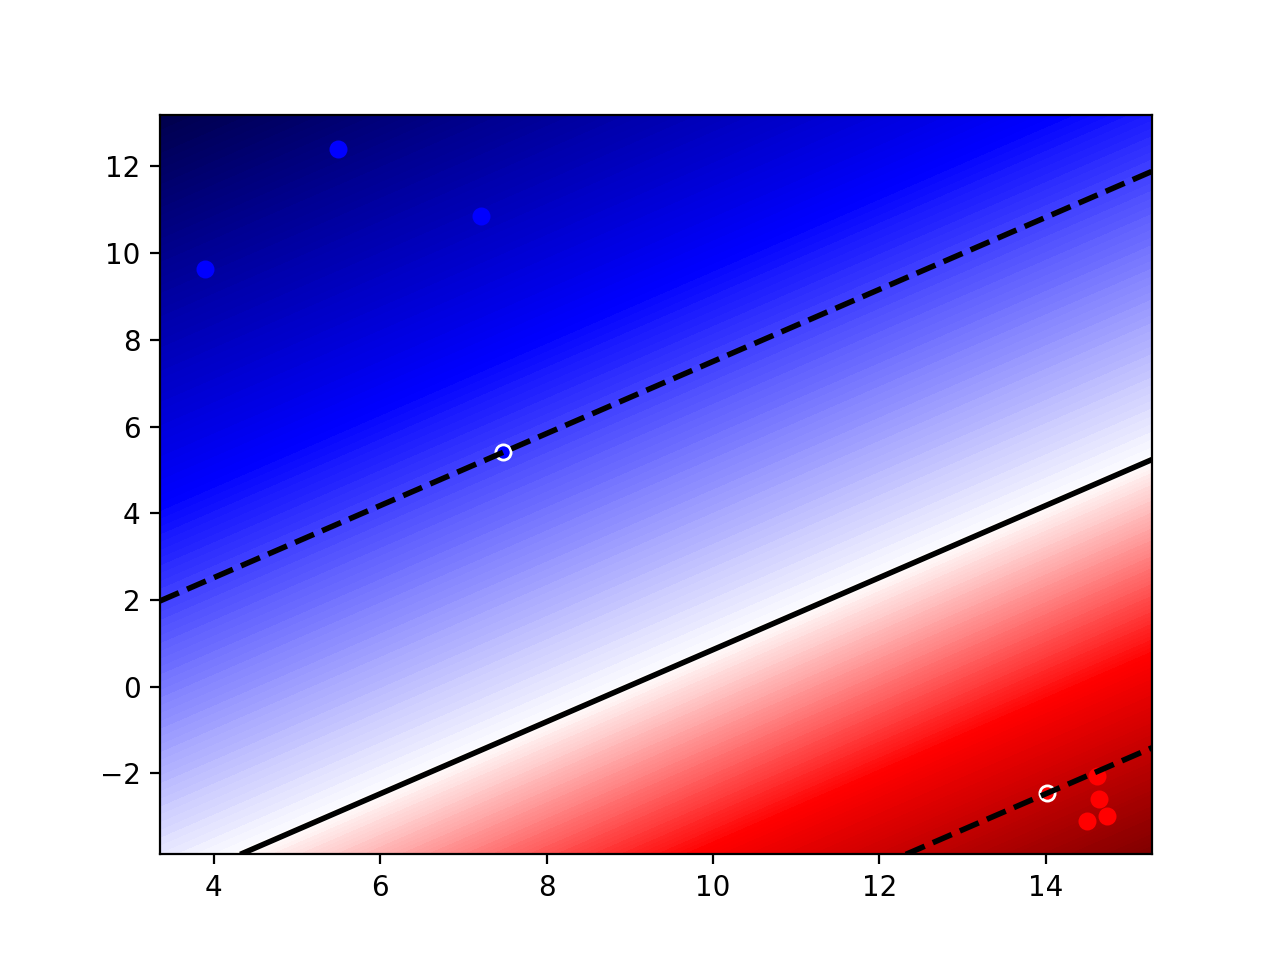
\includegraphics[width=\textwidth]{recursos/3/svm_small}
        \caption{SVM}
    \end{subfigure}
     \caption{Plots of what the linear decision boundary looks like when classification is performed in 2D after PCA dim. reduction }
\end{figure}




\subsection{Decoding the message from the Heavens}
To decode the message we simply run a map over the 'Xte\textunderscore digits\textunderscore 2017.mat' data set, using the classification function from our selected classifier, in our case LMS. This will turn the array of feature vectors into an otherwise equal array containing labels. Next we feed that vector into the 'y2ascii' function that we conveniently have on hand. We could do preliminary PCA, to reduce dimension, but the LMS algorithm should handle it. Doing this we get out the following message:

\begin{center}
\begin{verbatim}
i#guess#that#if#you#can#decode#this#messagee#
you#must#be#a#pretty#good#student#in#
fys#thirtytwelve#pattern#recognition#
buckle#up#for#the#long#hour##of#programming#for#
this#home#examm#and#good#luck!. 
\end{verbatim}

\end{center}

That's nice.

\subsection{Conclusion }
Because of the clear linear separability of this data, all classifiers did exidingly well. This is good in the sense that one chan choose a simple classifer (LS,Bayes) that requires small amounts of computational power and runs quickly, as opposed to SVM and networks which are quite time consuming to train. The message was indeed decoded.









\section{ Appendix A: Code}
\subsection{About}
All of the code and present state of the analysis is located in the GitHub repo: \href{https://github.com/arthurnoerve/UiT-FYS3012-Home-Exam}{arthurnoerve/UiT-FYS3012-Home-Exam}. If any of this material has to be removed based on intelectual rights or similar, please tell me. The beef of the code is in the alpha package: "alpha.py". Here there are functions that do most of the things we have been doing here. They include: functions to find weights through for the LMS, LS, SMO and Bayes classifiers, generate 2LP networks (stored in their own datatype, a named tuple called twolp), load a given network from file, classify and test using a given network/classifer. There's also a function called 'fan' which basically goes through a range of values for a function, plots them and returns the min/max arg value based on whether the mode is set to max or min. The PCA function is also stored in this package. The main file used for data exploration and plot generation is 'main.py', 'pca.py' was used to generate and store the PCA transformation matrices. Included with this report is the code for the alpha package itself.

\subsection{The Alpha package code}
\lstset{    language=Python,
            breaklines=true,
            caption=The alpha package,
            keywordstyle=\color{blue},
            stringstyle=\color{red},
            commentstyle=\color{black}
            }
\begin{framed}
\lstinputlisting{recursos/alpha.py}
\end{framed}



\newpage
%STuff:





\end{document}













